%!TEX root = ../document.tex
\chapter{Lösungsansatz} \label{chp:Loesungsansatz}
	In diesem Kapitel wird ein Verfahren zur Georeferenzierung von Twitter-Nutzern vorgestellt.
	Die Fragestellungen aus Kapitel \ref{sec:fragestellung} werden, unter Berücksichtigung der Anforderungen aus Kapitel \ref{sec:Anforderungen}, beantwortet.  

	Im Überblick soll zunächst gezeigt werden wie die Georeferenzierung abläuft und wie dies im realisiert werden kann.
	Danach soll eine generelle Struktur einer Datenbasis zur Georeferenzierung vorgestellt werden.
	In den darauffolgenden Abschnitten wird ganz allgemein betrachtet welche Eigenschaften geografische Indikatoren haben müssen um eine Georeferenzierung zu ermöglichen.
	\footnote{Unter einem geografischen Indikator wird ein Datum verstanden welches einen geografischen Bezug aufweist, sodass eine Georeferenz abgeleitet werden kann.}
	Danach sollen der Nutzer-Standort und die Nutzer-Zeitzone als mögliche geografische Indikatoren aus Twitter eingehender betrachtet werden. 
	Basierend darauf soll dann ein Verfahren zum einlernen der Datenbasis zur Georeferenzierung erarbeitet werden.
	Dabei wird auch die Struktur der Datenbasis weiterentwickelt.
	Zum Schluss wird ein Verfahren zur Georeferezierung vorgestellt.
	Es wird dazu die zuvor erarbeitete Datenbasis genutzt. 

	\section{Überblick} \label{sec:ueberblick} 
		
		Das erarbeitete Verfahren soll es ermöglichen Twitter-Nutzern eine Georeferenz zuzuordnen.
		Dabei sollen als Eingabe für die Georeferenzierung geografische Indikatoren aus dem Profil eines Twitter-Nutzers verwendet werden.
		Als Ergebnis soll eine Georeferenz zurückgeliefert werden. 
		Dabei hat der Anwender die Möglichkeit einen Schwellwert für die Konfidenz der Georeferenz anzugeben.
		Zudem kann der Nutzer die gewüschte geografische Hierarchiebene der zurückgelieferten Georeferenz angeben. 
		In Abbildung \ref{img:GeoreferenzierungAllg} ist der generelle Ablauf dieser Georeferenzierung dargestellt. 
		\todo{Schema Darstellung Eingabe->Ausgabe  Sketchbook A1: Unterschrift Die Eingabe besteht aus dem Nutzer-Standort sowie der Nutzer-Zeitzone. 
		Als Rahmenbedingungen wird die gewünschte Hierarchieebene sowie der Schwellwert für die Konfidenz angeben. 
		Als Ausgabe erhält man eine Georeferenz} 

		\begin{figure}[h!]
			\begin{center}
				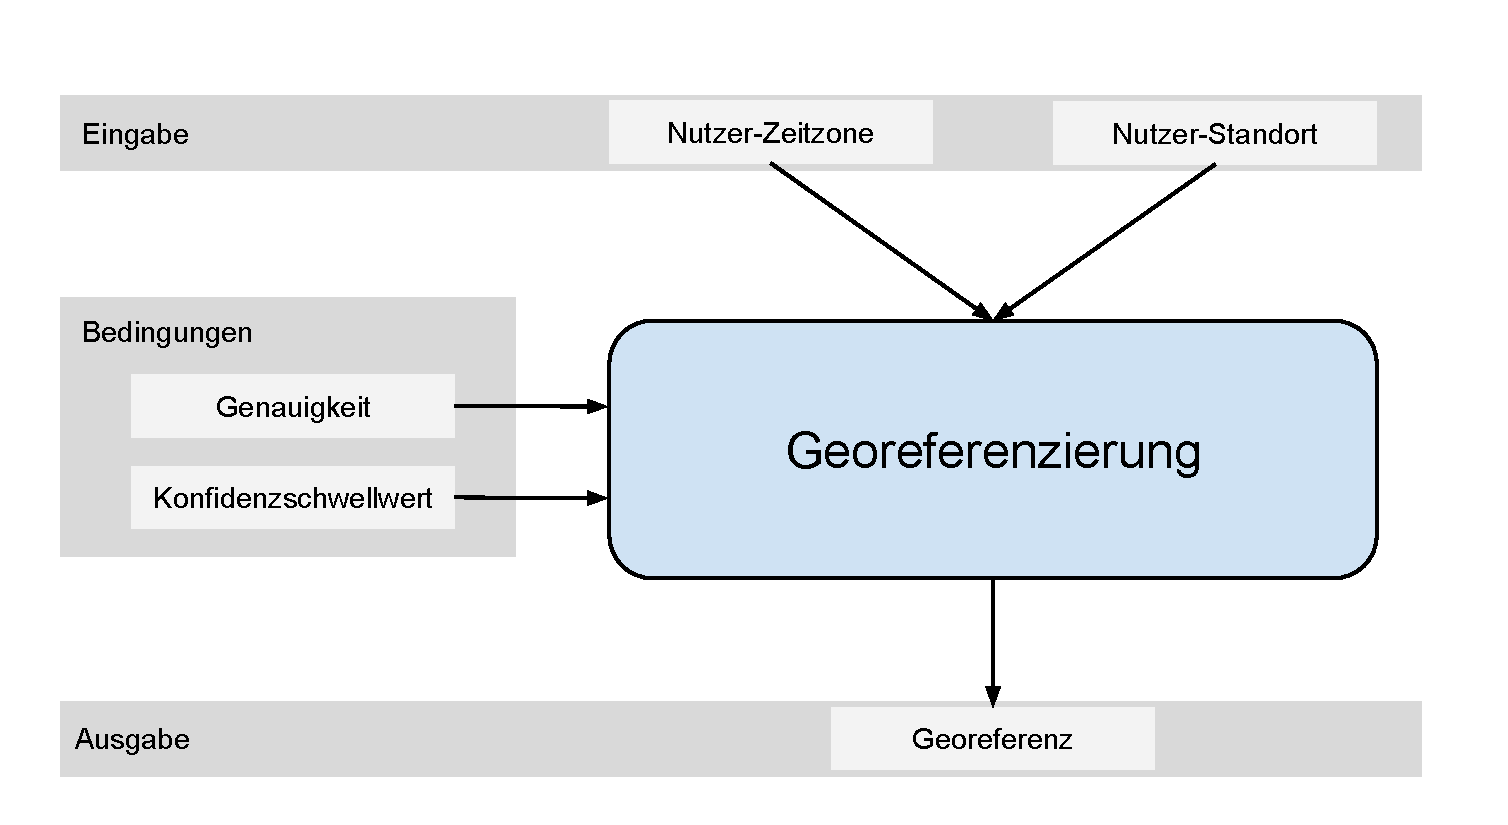
\includegraphics[scale=0.5]{A1.pdf}
				\caption{Ablauf Georeferenzierung}
				\label{img:georef}
			\end{center}
		\end{figure}	

		Die Georeferenzierung nach dem Schema aus Abbildung \ref{img:georef} setzt voraus, dass aus den eingegebenen geografischen Indikatoren eine Georeferenz abgeleitet werden kann.     
		Dies ist mit einer Datenbasis, die zu einem gegebenen geografischen Indikator eine Georeferenz liefern kann möglich.
		Aus einer Tweet-Datensammlung soll die Zuordnung der geografischen Indikatoren zu einer Georeferent gelernt werden.
		Die Tweet-Datensammlung enthält eine Menge von Tweets für welche die genutzten geografischen Indikatoren des Verfassers und eine Georefenz in Form von Längen- und Breitengrad angegeben sind.
		Die gelernten Zuordnungen sollen in einer Datenbasis gespeichert werden.
		Diese Datenbasis wird Georeferenz-Basis genannt.

		\todo{img:georef, img:ablaufEinlernen, img:Georeferenzierung} 

	\section{Generelle Struktur einer Georeferenz-Basis zur Georeferenzierung} \label{sec:generelleStruktur} 

		In diesem Kapitel soll eine generelle Struktur angegeben werden, welche die minimalen Anforderungen einer Georeferenzierung erfüllen kann.
		Danach wird das Schema und die nötigen Informationen, welche die Georeferenz-Basis beinhaltet, genauer betrachtet.
		
		Nach Abbildung \ref{img:allgA1} wird bei der Georeferenzierung einem oder mehreren geografischen Indikatoren eine Georeferenz zugewiesen.
		In der einfachsten Variante wird lediglich ein einziger geografischer Indikator an die Georeferenzierung übergeben und genau eine Georeferenz zurückgegeben.
		Die Georeferenzierung muss also zu einem gegebenen geografischen Indikator eine Georeferenz bestimmen können.
		Dies führt zu einer ersten einfachen Struktur für die Georeferenz-Basis.	

		\subsection*{Eine erste einfache Struktur der Georeferenz-Basis} 

			Es wird angenommen der geografische Indikator stellt immer ein eindeutiges Toponym dar.
			Des weiteren sind alle möglichen Toponyme sowie eine zugehörige Georeferenz bekannt. 
			Die Georeferenz liegt als Adresse mit Straße, Hausnummer, Postleitzahl und Ortsname vor.

			Jedem möglichen Toponym, welches im gegebenen geografischen Indikator vorkommen kann, soll eine Georeferenz zugeordnet werden können. 
			Daraus ergibt sich die Anforderung, dass die Georeferenz-Basis eine Menge von Datensätzen beinhalten muss, die jeweils aus einem Toponym und einer Georeferenz bestehen.
			Dieser Aufbau entspricht einer Art Wörterbuch in dem Informationen zu einem gegebenen Referenzwert nachgeschlagen werden können.
			Im vorliegenden Fall kann also zu einem Toponym die enstprechende Georeferenz nachgeschlagen werden.
			Die Referenzwerte stellen dabei mögliche Werte für den geografischen Indikator dar. 
			In Abbildung \ref{tab:simpleStruktur} ist ein Beispiel für eine sehr simple Struktur dargestellt.

			\begin{table}[htpb]
					\caption{Erste einfache Struktur für eine Georeferenz-Basis zur Georeferenzierung} 
					\centering
					\begin{tabular}{|c|c|}
						\hline
						Referenzwert & Georeferenz \\
						\hline\hline
						Zoo-Karlsruhe & Ettlinger Straße 6 - 76137 Karlsruhe \\
						\hline
						ZKM & Lorenzstraße 19 D - 76135 Karlsruhe \\
						\hline
						Elbphilharmonie & Dammtorwall 46 - 20355 Hamburg \\
						\hline
					\end{tabular}
					\label{tab:simpleStruktur} 
			\end{table} 

			Wird eine Abfrage auf die Georeferenz-Basis mit den geografischen Indikatoren "'Zoo-Karlsruhe"', "'ZKM"' oder "'Elbphilharmonie"' durchgeführt, kann nun eine Georeferenz zurückgeliefert werden.
			Diese simple Struktur reicht grundsätzlich aus um eine Georeferenzierungen durchführen zu können.
			In dem angeführten Beispiel ist die Menge der möglichen Toponyme sehr begrenzt, aber diese kann beliebig erweitert werden.
			Damit können sehr mächtige Datenbanken erstellt werden.

			Es sollen nun der Referenzwert und die Georeferenz genauer betrachtet werden.

			\paragraph{Form der Georeferenz}

				Die Form in der die Georeferenz angegeben wird ist abhängig von der Anwendung. 
				Im Beispiel \ref{tab:simpleStruktur} wurden Adressen verwendet. 
				Dazu muss das angegebene Toponym oder die Zeichenkette jedoch eine Adresse besitzen. 
				Ein See in der Wildnis Alaskas wird keine solche Adresse aufweisen.
				Aber auch die geografische Position einer Stadt oder eines Landes kann nicht durch eine Adresse beschrieben werden. 
				Die Form in der die Georeferenz angegeben wird kommt auf den jeweiligen Anwendungsfall an.
				Denkbar sind hier unter anderem:

				\begin{itemize}
				  	 \item geografische Koordinaten
				  	 \item vollständige Adressen
				  	 \item Ländernamen
				  	 \item Städtename
				  	 \item Namen adminsitrativer Verwaltungsgebiete 
				  	 \item Zeitzonen
				  	 \item ein Straßenname und eine Kilometerbezeichnung
				  \end{itemize}  

				  Grundsätzlich sind alle Formen, welche eine direkte oder indirekte Georeferenz darstellen, denkbar.
				  Wichtig ist nur, dass die Angabe der Georeferenz in einer Form erfolgt, welche für die gegebene Anwendung ausreichend genau ist.

				  Für den Straßenverkehr ist eine Angabe einer Adresse ausreichend.
				  Für Wanderungen in unerschlossenen Gebieten hingegen sind geografische Koordinaten notwendig. 

			\paragraph{Form der Referenzwerte}

				Der Referenzwert ergibt sich aus den möglichen Werten der Indikatoren.
				Die Indikatoren sind dabei zumeist Zeichenketten.
				Abhängig vom Indikator können diese Zeichenketten verschiedene Informationen enthalten.
				Im obigen Beispiel sind die Referenzwerte Toponyme.
				Toponyme sind Namen für geografische Objekte, es kann ihnen also unmittelbar ein geografisches Objekt zugeordnet werden.
				Es muss sich dabei aber nicht um Toponyme handeln.
				Werte die als Referenzwerte in Frage kommen sollen als geografische Indikatoren bezeichnet werden.
				Toponyme sind also geografische Indikatoren, da sie direkt mit einem geografischen Objekt in Verbindung gebracht werden können.
				Geografische Indikatoren können aber auch indirekt mit einem geografischen Objekt in Verbindug gebracht werden.
				Unbrauchbar sind Werte welche weder direkt noch indirekt mit einem geografischen Objekt in Verbindung gebracht werden können.
				Diese Werte stellen keine geografischen Indikatoren dar.
				Im nächsten Abschnitt werden die geografischen Indikatoren genauer betrachtet.

	\section{Geografische Indikatoren} 

		Ein geografischer Indikator ist ein Datum welches einen geografischen Bezug aufweist.
		Es sind also genau die Werte, welche in irgendeiner Weise mit einem geografischen Objekt in Verbindung gebracht werden können.

		Geografische Indikatoren können unmittelbaren geografischen Bezug oder mittelbaren geografischen Bezug haben. 

			\subsection{Indikatoren mit unmittelbarem geografischen Bezug} \label{subsec:unmittelbareGeografischeIndikatoren} 

				Ein geografischer Indikator mit unmittelbarem geografischen Bezug beschreibt direkt eine geografische Position oder eine geografische Region.	
				Dem geografischen Indikator kann durch die in ihm enthaltene Information direkt eine Georeferenz auf ein geografisches Objekt zugewiesen werden. 

				Im Beispiel in Tabelle \ref{tab:simpleStruktur} wurden geografische Indikatoren mit unmittelbarem geografischen Bezug verwendet. \todo{XXX->wenn in Grundlagen soll} 
				Die Referenzwerte entsprechen Toponymen, diese sind Namen für geografische Objekte. 
				Ihnen kann also unmittelbar ein geografisches Objekt zugeordnet werden.

				Ein weiteres Beispiel für geografische Indikatoren mit unmittelbarem geografischen Bezug sind Zeitzonen.

				Bei der Zeitzone handelt es sich um einen geografischen Indikator der eine geografische Region beschreibt.
				Die zugehörige Georeferenz für eine Zeitzone könnten die Länder sein welche die Zeitzone umfasst. 
				Aber auch die Kontinente oder Städte welche in dieser Zeitzone liegen könnten, je nach Anwendugsfall, von Interesse sein.

			\subsection{Indikatoren mit mittelbarem geografischen Bezug} 

				Ein geografischer Indikator muss nicht unmittelbar einer Georeferenz zuzuordnen sein.
				Dies ist genau dann der Fall, wenn die im geografischen Indikator enthaltene Information nicht direkt auf ein geografisches Objekt hindeutet.
				
				An einem Beispiel soll gezeigt werden was einen geografischen Indikator mit mittelbarem geografischen Bezug ausmacht.
				
				\paragraph{Beispiel eines mittelbaren geografischen Indikators} 
				In einem Feld auf einer Website werden die Nutzer nach alternativen Begriffen für Kartoffeln gefragt. 
				Die folgenden drei Begriffe werden eingegeben.

				\begin{enumerate}
				 	\item Äbierra
				 	\item Grumbeer
				 	\item Tüfte 
				 \end{enumerate} 

				Die Information die hinter jedem dieser Begriffe steckt ist die Bezeichnung eines Gemüses.
				Die Begriffe bezeichnen also insbesondere kein geografisches Objekt und haben somit keinen unmittelbaren geografischen Bezug.
				Jede dieser Bezeichnungen stammt aber aus unterschiedlichen Regionen Deutschlands, denn es handelt sich um dialektiche Begriffe.
				Durch ihre geografisch begrenzte Verwendung können sie damit einer geografischen Region zugeordnet werden.
				Durch die Verwendung eines dieser Worte kann also auf eine Region Deutschlands geschlossen werden.
				Dadurch kann jedem Begriff eine Georeferenz zugewiesen werden.

				Mit folgender Georeferenz-Basis kann eine Georeferenzierung der obigen Begriffe durchgeführt werden:

				\begin{table}[htpb]
					\caption{Kartoffeln in verschiedenen Dialekten} 
					\centering
					\begin{tabular}{|c|c|}
						\hline
						Referenzwert & Georeferenz \\
						\hline\hline
						Äbbiera & Württemberg \\
						\hline
						Grumbeer & Pfalz \\
						\hline
						Tüfte & Norddeutschland \\
						\hline
					\end{tabular}
					\label{tab:dialekt} 
				\end{table} 

				In diesem Beispiel wurde die Zuordnung zu einem geografischen Objekt über die Verwendung der Begriffe in bestimmten Regionen ermöglicht.
				Aber auch andere Informationen können dazu dienen einem Indikator eine Georeferenz zuzuordnen.
				Es kommt grundsätzlich nicht darauf an was genau mit dem Begriff bezeichnet wird. 
				Lediglich die geografisch begrenzte Verwendung kann hier als Hinweis auf eine Georeferenz dienen. 

	\section{Toponyme als geografische Indikatoren} \label{sec:topGeogInd} \todo{XXX->Annahmen raus, können nicht merh verwendet werden} 

		Toponyme sind die am häufigsten auftretende Art geografischer Indikatoren. 
		Es handelt sich dabei um geografische Indikatoren mit unmittelbarem geografischen Bezug.

		Die Georeferenzierung von Toponymen kann bereits mit der Struktur aus Tabelle \ref{tab:simpleStruktur} umgesetzt werden. 
		Jedes Toponym wird dabei als Referenzwert gespeichert und eine Georeferenz zugewiesen.
		Es wurden allerdings mehrere Annahmen gemacht, die in der Regel nicht gelten.
		Anhand dieser Annahmen soll auf die Probleme bei der Verwendung von Toponymen als geografische Indikatoren eingegangen werden. 

		\subsection{Probleme bei der Verwendung von Toponymen} 

			Im folgenden soll auf diese Annahmen eingegangen werden und gezeigt werden wieso diese im Allgemeinen nicht gelten.
			Des weiteren werden generelle Probleme bei der Verwendung von Toponymen zur Georeferenzierung aufgezeigt.

			\subsubsection{Alle möglichen Toponyme sind bekannt}

				Es existieren sehr umfangreiche Datenbanken, die Toponymen Georeferenzen zuweisen.
				Eine dieser Datenbanken ist das frei erhältliche Ortsverzeichnis von geonames.org.
				Es beinhaltet ca. 8,9 Millionen Toponyme und zugehörige Georeferenzen.
				Zusätzlich sind weitere ca. 8 Millionen alternative Toponyme hinterlegt.
				In den Datensätzen sind neben einer Georeferenz in Form geografischer Koordinaten noch andere Informationen hinterlegt wie beispielsweise Länderkürzel und Einwohnerzahlen. 
				Auch eine geografische Hierarchie wird in der Datenbank abgebildet.
				Grundsätzlich ist die Datenbank aber nach obiger Struktur aufgebaut.

				Trotz der großen Anzahl an hinterlegten Toponymen beinhalten solche Datenbanken nicht alle möglichen Toponyme.
				Aufgrund der immensen Vielfalt ist es nahezu unmöglich alle Toponyme abzudecken. 
				Im folgenden soll an einigen Beispielen die Vielfalt der Toponyme belegt werden.

				\paragraph{Vielfalt der Toponyme} 

					Da Toponyme im allgemeinen nicht definiert sind, und neben den offiziellen Namen für Städte, Länder usw. weitere Namen vorkommen können, ist die Vielfalt nahezu unbegrenzt.
					
					In Wikipedia sind für die Stadt Detroit, im US-Bundesstaat Michigan, folgende Spitznamen angegeben:
					
					\begin{itemize}
						\item The Motor City
						\item Motown
						\item Hockeytown
						\item Rock City
						\item The D
					\end{itemize}

					Die ersten zwei dürften weltweit einen Gewissen Bekanntheitsgrad haben. 
					Hockeytown, Rock City und The D dürften allerdings weniger bekannt sein.
					Tatsächlich beinhaltet die geonames.org Datenbank keinen dieser Spitznamen.
					Google Maps hingegen bietet bei Eingabe der oben genannten Spitznamen Detroit als Vorschlag an.

					Das Problem wird noch gravierender wenn man lokal begrenzte Spitznamen einbezieht.
					Es ist durchaus denkbar, dass Spitznamen für einen Stadtteil nur lokal verwendet werden und über die Stadt- oder Landesgrenze hinaus nicht bekannt ist. 
					Diese Spitznamen können nur schwer erfasst werden.
					Solche Spitznamen existieren auch für Länder und administrative Verwaltungsebenen. 

					Weitere Beispiele die zu einer größeren Vielfalt der Toponyme führen:

					\begin{itemize}
						\item Historische Toponyme
						\item Kulturell bedingte Toponyme
						\item Toponyme für landschaftliche Besonderheiten
						\item Toponyme für bestimmte Landschaften
					\end{itemize}
		
			\subsubsection{Die Toponyme sind eindeutig geografischen Objekten zuzuweisen und umgekehrt} 

					Auch dies ist im allgemeinen nicht der Fall. 
					Toponyme sind oft Doppel- oder Mehrdeutig und verweisen somit auf mehrere Georeferenzen.
					Allerdings können zu einer Georeferenz auch mehrere eindeutige Toponyme existieren.
					Doppel- und Mehrdeutigkeiten können also sowohl ausgehend von der Georeferenz, als auch ausgehend vom Referenzwert auftreten.

				\paragraph{Zu einem Referenzwert können mehrere Georeferenzen existieren}

					Es gibt zahlreiche Städte-Namen, die in mehreren Ländern verwendet werden.
					Ein gutes Beispiel hierfür sind US Städte. 
					Da die USA ein Einwanderungsland ist, übernahmen viele Einwanderer bei der Gründung neuer Städte die Namen aus der alten Heimat. 
					So finden sich in den USA zahlreiche Städte deren Namen exakt den deutschen Städtenamen entsprechen. 
					In Tabelle \ref{tab:usCitiesGemanNames} sind einige Städte-Namen und die Vorkommen in den USA aufgelistet.
					
					\begin{table}[htpb]
						\caption{Häufige deutsche Städtenamen in den USA} 
						\centering
						\begin{tabular}{|c|c|}
							\hline
							Name & Anzahl in den USA \\
							\hline\hline
							Hannover & 40 \\
							\hline
							Berlin & 39 \\
							\hline
							Hamburg & 30 \\
							\hline
						\end{tabular}
						\label{tab:usCitiesGermanNames} 
					\end{table}


					Soll nun eine Georeferenz-Basis angelegt werden, welche einem Stadt-Namen einen Staat zuweist müssten für Hannover 41, für Berlin 40 und für Hamburg 31 Georeferenzen hinterlegt sein.
					Als Ergebnis einer Georeferenzierung für den Wert "'Hamburg"' würden 31 Georeferenzen in den USA und eine in Deutschland zurückgegeben werden. 

					Diese Mehrdeutigkeit stellt ein Problem bei der Georeferenzierung dar.
					Es kann keine eindeutige Entscheidung getroffen werden welche Georeferenz dem Ort zugewiesen werden soll. 

				\paragraph{Zu einer Georeferenz können mehrere Referenzwerte existieren}

					Dies wird anhand der Städte-Spitznamen klar. 
					Städte-Spitznamen sind oft eindeutig, allerdings kann eine Stadt mehrere dieser eindeutigen Spitznamen besitzen. 
					Damit ergibt sich eine Mehrdeutigkeit ausgehend von der Georeferenz zu einem Toponym.
					Dies ist grundsätzlich auf alle geografischen Objekte übertragbar.
					Zu jedem geografischen Objekt existieren potenziell mehrere gültige Toponyme.

					Das Problem hierbei stellt nicht die Beziehung der Georeferenz zu den Toponymen dar, sondern eher die vielfalt der Toponyme. 

		\subsection{Domänenspezifische Toponyme} 

			Ein weiteres Problem kann die untersuchte Domäne darstellen. 
			In sozialen Netzwerken können sich eigene Begriffe und Formulierungen etablieren welche im allgemeinen nicht bekannt sind.

			Im Twitter-Umfeld haben sich in den letzten Jahren beispielsweise einige spezielle Begriffe und Formulierungen zur Verwendung in Tweet-Texten etabliert. 
			Das im Twitter-Umfeld spezielle Toponyme verwendet werden, kann nicht gänzlich ausgeschlossen werden. 

			Ein Beispiel hierfür ist "'Bieberville"' welches in den untersuchten Daten von Hecht et al. öfter vorkommt.
			"'Bieberville"' wird abgeleitet von dem Pop-Star Justin Bieber.	
			Twitter wird oft als "'Bieberville"' bezeichnet, da der Pop-Star in Twitter sehr aktiv ist und deshalb viele Fans auch in Twitter aktiv sind.
			Unter diesem Gesichtspunkt hätte "'Bieberville"' keinen geografischen Bezug.
			Sucht man allerdings im Internet nach "'Bieberville"' stößt man auf einen Imbiß in Groß-Bieberau.
			"'Bieberville"' kann also durchaus einen geografischen Bezug haben, wenngleich es im Twitter-Umfeld nicht als solcher benutzt wird. 
			Ein Nutzer-Standort der in einem Land kein Toponym darstellt, kann in einem anderen durchaus ein Toponym sein.

			Die Benutzung von "'Bieberville"' könnte auch ein temporäres Phänomen darstellen. 
			In den Tweet-Daten welche für diese Arbeit verwendet werden befindet sich kein Eintrag mit dem Nutzer-Standort "'Bieberville"'.
			Dies könnte ein Hinweis auf eine temporäre Verwendung des Begriffes im Nutzer-Standort sein.
			Leider ist es nicht möglich Nutzer nach dem Nutzer-Standort zu suchen und deshalb kann diese Aussage nicht mit Sicherheit getroffen werden. 
			Gibt es Toponyme die tatsächlich nur temporär auftauchen wird das Problem noch größer. 
			Dies ist durchaus denkbar, denn mit wenigen Klicks und einer kurzen Eingabe kann der Nutzer-Standort geändert werden.

			Das Wissen über solche Begriffe und Formulierungen kann nur sehr schlecht erfasst werden, wenn man die enstprechende Domäne nicht untersucht. 


			\todo{Bieberville beispiel in lernen} 

		\subsection{Fazit}

			Es existieren sehr umfangreiche Datenbasen um Toponymen eine Georeferenz zuzuweisen. 
			Toponyme unterliegen grundsätzlich keiner Kontrolle und sind nicht standardisiert womit der Veilfalt keine Grenzen gesetzt sind.
			Es ist schwer, wenn nicht sogar unmöglich, das Wissen über geografische Objekte und deren zugehörige Toponyme vollständig zu erfassen.
	
	\section{Der Nutzer-Standort} \label{sec:nutzerStandort} 

		Der Nutzer-Standort eines Twitter-Nutzers soll als geografischer Indikator verwendet werden.
		Bei der Eingabe des Nutzer-Standortes wird vom Nutzer abgefragt, wo dieser sich befindet. 
		Die Intention der Abfrage zielt also darauf ab, dass der Nutzer einen Wert eingibt der auf ein geografisches Objekt verweist, welches seinem Standort entspricht. 
		Es ist naheliegend, dass der Nutzer seinen Standort mit Hilfe eines Toponyms angibt.
		Der Nutzer-Standort wird jedoch vom Nutzer frei eingegeben und unterliegt keinerlei Kontrolle.
		Dieser muss also nicht zwangsweise Werte mit geografischem Bezug enthalten. 

		Da allerdings Toponyme zu erwarten sind, können alle in Kapitel \ref{sec:topGeogInd} erwähnten Probleme auftreten.
		Durch die unkontrollierte Eingabe sind tatsächlich alle möglichen Toponyme denkbar.
		Aber auch geografische Indikatoren mit mittelbarem geografischem Bezug oder Werte ohne geografischen Bezug können im Nutzer-Standort angegeben werden.		

		Hier soll nun der Nutzer-Standort genauer betrachtet werden und ob dieser überhaupt zur Erzeugung geografischer Indikatoren geeignet ist.

		\subsection*{Geografischer Bezug des Nutzer-Standorts?} 
			
			Nach Hecht et al. haben in \cite{Hecht2011} den Nutzer-Standort eingehend untersucht und sind zu folgendem Ergebnis gekommen:
			Wenn der Nutzer überhaupt einen Standort angegegeben konnte in 80\% Prozent der Fälle ein geografischer Bezug nachgewiesen werden.
			In den restlichen 20\% der Fälle konnte im Nutzer-Standort kein geografischer Bezug nachgewiesen werden. 
			Die Untersuchung wurde manuell vorgenommen und es durften alle zur Verfügung stehenden Mittel zur Analyse der Daten verwendet werden. 
			Hecht et al. haben deshalb ausschließlich Daten untersucht die nachweislich aus den USA stammten. 

			Es kann hier also festgehalten werden, dass 80\% der Nutzer-Standorte als geografischer Indikator verwendet werden können.
			Es muss bechtet werden, dass nur Daten aus den USA betrachtet wurden.

			Im Rahmen der vorliegenden Arbeit wurde der Nutzer Standort von 1000 Twitter-Nutzern ebenfalls manuell untersucht. \footnote{siehe \ref{chp:AppendixA} }  
			Dabei wurde keinerlei Einschränkung zur Herkunft gemacht.
			Um zu prüfen ob ein geografischer Bezug vorliegt und eine Georeferenz zuzuordnen wurden Ortsverzeichnisse von Google-Maps und Geonames.org verwendet.
			Diese lassen es zu auch Nutzer-Standorte die in unbekannten Sprachen und Alphabeten verfasst wurden zu untersuchen.
			Es konnte dabei in 76\% der Fälle ein geografischer Bezug nachgewiesen werden. 

			In den restlichen 24\% der Fälle konnte kein geografischer Bezug mit Hilfe der Datenbanken nachgewiesen werden. 
			Dies bedeutet nicht, dass grundsätzlich kein geografischer Bezug vorhanden ist. 
			Es konnte lediglich anhand der genutzten Quellen kein geografischer Bezug hergeleitet werden.
			Beispielsweise wurde "'Swag City"' nicht zugewiesen, denn der Spitzname für die Stadt Ann Arbor war in den Datenbanken nicht hinterlegt. 

			Der Nutzer-Standort kann also in vielen Fällen einen Hinweis auf die Herkunft des Twitter-Nutzers geben.
			Bei der durchgeführten Untersuchung wurden insbesondere nur Toponyme und damit geografische Indikatoren mit unmittelbarem geografischen Bezug identifiziert. 

		\subsection*{Genauigkeit der geografischen Angaben}

			In ca. 80\% der Fälle kann bei einer Angabe des Nutzer-Standortes davon ausgegangen werden, dass dieser geografischen Bezug hat.
			Wiederum aufgrund dessen, dass der Nutzer beliebige Eingaben machen kann, ist nicht sicher wie genau ein solcher geografischer Bezug ist. 
			
			Hecht et al. analysierten ihre Daten auch darauf wie genau die Nutzer ihren Standort angeben.
			Dabei ist wiederum zu beachten, dass die Daten aus den USA stammen und deshalb die geografischen Verwaltungsebenen der USA zugrunde gelegt wurden.
			Dabei wurden folgende Werte festgestellt:

			\begin{itemize}
			 	\item 64\% Stadt 
			 	\item 20\% Staat (Adminstrationsebne erster Ordnung) 
			 	\item ca. 8\% Intrastate (Adminstrationsebene zweiter Ordnung) 
			 	\item ca. 5\% Land 
			 \end{itemize} 

			 Die restlichen 13\% entfallen auf Interstate Regionen, Nachbarschaften und konkrete Adressen. 
			 Interstate Regionen sind Regionen die sich über mehrere Staaten hinwegziehen. 
			 Beispiele für Interstate Regionen sind "'Central United States"' oder "'West-Coast"'.
			 Nachbarschaften(Neighbourhoods) sind oft Stadtteile wie "'Harlem"' oder "'Bronx"' in New York.

			 In den eigenen Untersuchungen sind folgende Werte (gerundet) festgestellt worden:

			\begin{itemize}
			 	\item 77\% Stadt %593
			 	\item 8\% Adminstrationsebene erster Ordnung %63
			 	\item 4\% Adminstrationsebene zweiter Ordnung %34
			 	\item 10 \% Land %79 gesamt 769
			 \end{itemize} 

			Es ist also, selbst wenn ein geografsicher Bezug besteht, nicht sicher welcher geografischen Hierarchiebene dieser zugeordnet werden kann. 
			Die unterschiedlichen Ergebnisse können dadurch Zustande kommen, dass sich Hecht et al. auf Tweets aus den USA beschränkt haben.  


		\subsection*{Stimmt der tatsächliche Standort mit dem angegeben überein?}

			Diese Frage ist grundsätzlich nur schwer zu beantworten.
			Die einzige Möglichkeit besteht darin Tweets mit geografischen Angaben zu untersuchen.
			Dabei können aber Probleme auftreten. 
			Der Nutzer-Standort gibt oft nicht den Aufenthaltsort sondern den Heimatort an. 
			Befindet sich der Nutzer auf Reisen oder arbeitet er in einer anderen Stadt korrespondiert die gegrafische Koordinate nicht mit dem angegeben Ort.
			Dies könnte in einige Fällen gelöst werden indem mehrere Tweets desselben Nutzers über einen längeren Zeitraum untersucht werden. 
			Um den eigentlichen Wohnort sollte dadurch eine Häufung an abgesetzten Tweets auftreten.
			Damit kann ein genauerer Standort bestimmt werden.
			Der Nutzer kann aber auch absichtlich einen falschen Standort angeben oder bei Umzug in eine andere Stadt oder ein anderes Land schlicht vergessen haben den Nutzer-Standort anzupassen.

			In der durchgeführten Untersuchung wurde fesgestellt, dass auf Städtebene 60\% der Tweets in weniger als 24 Kilometern Entfernung von der manuell ermittelten Stadt abgesetzt wurden.
			25\% der Tweets sind aber mehr als 239 Kilometer von der Manuell ermittelten Stadt entfernt. 
			Der Median liegt bei 11 Kilometern.
			In Tabelle \ref{tab:distancesP} sind weitere Informationen über die Distanzen zusammengetragen.

			\begin{table}[h]
			\centering
			\caption{Distanzen}
			\label{tab:distancesP}
			\begin{tabular}{|l|l|}
			\hline
			Median       & 11,5  \\ \hline
			0,25 Quantil & 3,1   \\ \hline
			0,50 Quantil & 11,5  \\ \hline
			0,60 Quantil & 24,3  \\ \hline
			0,75 Quantil & 239,0 \\ \hline
			\end{tabular}
			\end{table}

			%6625.059088      11491.29743       24281.1066      106942.0694
			%Hier manuelles Tagge rein! 

		\subsection*{Partieller geografischer Bezug des Nutzer-Standortes} \label{subsec:partiellerGeografischerBezug} 

			In einigen der Einträge konnte festgestellt werden, dass nur Teile der Einträge geografischen Bezug haben. 
			Oft wollen die Nutzer noch weitere Informationen geben, diese haben oft keinen Nutzen für eine Georeferenzierung. 
			In der folgenden Liste sind einige Einträge von Nutzer-Standorten aufgelistet. 

			\begin{enumerate}
				\item 11th Dimension | California
				\item between here and there - Miami
			\end{enumerate}

			Im ersten Fall kann für Kalifornien ein geografischer Bezug festgestellt werden.
			11th Dimension hat hier offensichtlich keinen geografischen Bezug.
			Im zweiten Fall ist die Aussage "'between here and there"' nicht zu gebrauchen, Miami kann jedoch als Bezug zur Stadt Miami in Florida, USA gebracht werden.
			
			Es können also auch nur Teile des Nutzer-Standorts für eine Georeferenzierung von Nutzen sein.


		\subsection*{Wiedersprüchliche Werte im Nutzer-Standort} \label{subsec:wiederspruechlicheBezuege} 

			Es existieren auch Einträge für Nutzer-Standorte welche mehrere wiedersprüchliche Angaben machen.
			Das bedeutet es werden zwei oder mehr Werte mit geografischem Bezug angegegeben.

			Auch hier sollen einige Beispiele genannt werden:

			\begin{itemize}
				\item Bolton\textbackslash/Leigh
				\item Liverpool\textbackslash/London
				\item  Balikesir \textbackslash/ Izmir	
			\end{itemize}							
				
			In diesen Beispielen sind jeweils zwei Städte angegeben.
			Bolton und Leigh liegen 14km auseinander.
			Liverpool und London trennen ca. 350km.
			Balikesir und Izmir ca. 180km.

			Es kann nun spekuliert werden wieso der Nutzer zwei Städte angibt.
			Ist er in einer Stadt aufgewachsen und lebt momentan in der anderen?
			Pendelt er zwischen den Städten um zu arbeiten?

			Wie dem auch sei, es kann nicht eindeutig entschieden werden in welcher Stadt sich der Nutzer aufhält.


		\subsection*{Geografische Hierarchien im Nutzer-Standort}

			Es ist auch möglich das im Nutzer-Standort teile einer geografischen Hiararchie angegeben sind.
			Die Angabe von Stadt in Kombination mit einem Land.
			In den USA wird auch oft die Stadt und der zugehörige Bundesstaat angegeben.
			Hier einige Beispiele:

			\begin{itemize}
				\item Los Angeles, California
				\item Mato Grosso, Brazil
				\item Bronx, New York	
			\end{itemize}		

			Im ersten Beispiel handelt es sich um die Stadt Los Angeles und den US-Bundesstaat Kaliforniern.
			Im zweiten Beispiel wird zuerste ein brasilianischer Bundesstaat angegeben und danach das Land.
			Im dritten Beispiel wird ein Stadtteil von New York angegeben und dann die Stadt oder der US-Bundesstaat. 
			Da der US-Bundesstaat denselben Namen hat wie die Stadt, und beide in einer Hierarchiebeziehung mit Bronx stehen, kann hier nicht unterschieden werden was gemeint ist.
			

		\subsection{Fazit}

			Der Nutzer-Standort eignet sich besonders gut als geografischer Indikator, allerdings sind die Eingaben nicht standardisiert und können somit nicht ohne Vorverarbeitung verwendet werden.
			Wie oben dargestellt kann der Nutzer-Standort nur partiellen geografischen Bezug haben oder mehrere Informationen verschiedener geografischer Hierarchieebenen beinhalten. 
			Auch kann der Nutzer-Standort keinen geografischen Bezug haben.
			Dies macht es grundsätzlich schwierig den Nutzer-Standort direkt als geografischen Indikator zu verwenden.
			Der Nutzer-Standort ist genaugenommen nur ein potenzieller geografischer Indikator, da nicht mit Sicherheit gesagt werden kann ob ein geografischer Bezug besteht oder nicht.
			Dies resultiert aus der völlig freien Eingabe durch den Nutzer.
			
			Ist ein geografischer Bezug des Nutzer-Standortes nachzuweisen, handelt es sich bei dem Eintrag in den meisten Fällen um ein Toponym.
			Durch die durchgeführte Untersuchung konnte gezeigt werden, dass ca. 76\% der Nutzer-Standorte mit einem geografischen Bezug, auf Toponyme zurückzuführen sind.
			Im Hinblick auf den geografischen Bezug der Einträge im Nutzer-Standort ergab sich kein signifikanter Unterschied zu den Untersuchugen von Hecht et al..

			Zusammenfassend kann gesagt werden, dass der Nutzer-Standort häufig einen geografischen Bezug aufweist und es sich in diesen Fällen um Toponyme handelt.
			Aufgrund der völlig freien Eingabe durch den Nutzer ergeben sich bei der Auswertung der Nutzer-Standorte jedoch einige Probleme die gelöst werden müssen.

	\section{Die Nutzer-Zeitzone}

		In Kapitel \ref{sec:topGeogInd} wurden auf die Probleme bei der Verwendung von Toponymen als geografische Indikatoren eingegangen.
		Dabei wurde die Doppel- und Mehrdeutigkeit von Toponymen betrachtet.
		Bei der Verwendung des Nutzer-Standortes kann dieses Problem auch auftauchen. 

		Um diesem Problem zu begegnen soll nun ein weiterer geografischer Indikator hinzugezogen werden, die Nutzer-Zeitzone.
		Zunächst sollen die generellen Eigenschaften der Nutzer-Zeitzone erläutert werden bevor erklärt wird wie die Nutzer-Zeitzone das Problem der Mehrdeutigkeit von Toponymen beheben kann.

		\subsection{Eigenschaften der Nutzer-Zeitzone}

			Die Nutzer-Zeitzone stellt einen unmittelbaren geografischen Indikator dar. 
			Sie beschreibt eine eindeutige geografische Region auf dem Globus.
			Dabei enstprechen die Grenzen der Region nicht unbedingt den Landesgrenzen oder den Grenzen sonstiger adminstrativer Verwaltungseinheiten. 
			In Abbildung \ref{img:timezones} sind die Zeitzonen der Erde dargestellt.

			\begin{figure}[h!]
				\begin{center}
					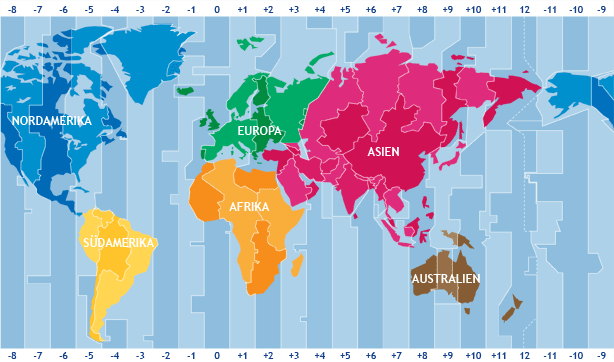
\includegraphics[scale=0.5]{zeitzonen_weltkarte.jpg}
					\caption{Zeitzonen der Erde. }
					\label{img:timezones}
				\end{center}
			\end{figure}	
			\todo{ Quelle: http://www.zeitzonen.de/images/frontend/mod\_tz\_map/zeitzonen\_weltkarte.gif} 

			Die Nutzer-Zeitzone kann in Twitter über eine Liste gewählt werden.
			\todo{Bild Auswahlliste} 
			Der Wert der Nutzer-Zeitzone stellt deshalb garantiert eine Zeitzone dar.
			Es ist dem Nutzer nicht möglich einen Wert einzugeben der nicht einer Zeitzone entspricht.

			Allerdings ist nicht gesichert, dass der angegegebene Wert auch der Zeitzone entspricht in der sich der Nutzer aufhält.
			Der Nutzer könnte eine bewusste Fehleingabe machen oder aber die Zeitzone nicht wählen womit der Stadardwert "'Pacific Time (US and Canada)"' gewählt wird.
			In Abbildung \ref{img:gephiTimezones} wurden Tweets anhand ihres Längen- und Breitengrades platziert.
			In der Abbildung sind Tweets aus den USA zu sehen. 
			Die Farben entsprechen den gewählten Zeitzonen.

			\begin{itemize}
			 	\item Pacific Time Blau
			 	\item Eastern Time	Rot
			 	\item Central Time Grün
			 	\item Mountain Time Pink 
			 \end{itemize} 

			 Die Zeitzonen sind durch die Farben gut zu erkennen. 
			 Lediglich die dünn besiedelte Region der Mountain Time kann nur an einigen Ballungszentren erkannt werden. 
			 Grundsätzlich scheint der Großteil der Angaben aber korrekt zu sein.

		\subsection{Auflösen von Doppeldeutigkeiten}

			Mit der Nutzer-Zeitzone lassen sich Doppeldeutigkeiten auflösen. 

			Besteht zu einem Nutzer-Standort eine Doppeldeutigkeit, kann nicht entschieden werden welches geografische Objekt zugeordnet werden soll.
			Liegen die beiden geografischen Objekte allerdings in zwei unterschiedlichen Zeitzonen und der Nutzer hat diese angegegeben kann die Doppeldeutigkeit aufgelöst werden indem zusätzlich die Zeitzone betrachtet wird.
			Somit kann dem Nutzer die korrelte Georeferenz zugewiesen werden.
			Vorausetzung dazu ist natürlich, dass die geografischen Objekte in zwei unterschiedlichen Zeitzonen liegen und die Nutzer-Zeitzone angegegeben ist.

	\section{Verfahren zum einlernen geografischer Indikatoren am Beispiel von Twitter} 

		Aus einer Tweet-Sammlung sollen die genutzten geografischen Indikatoren und deren Zuordnung zu einer Georeferenz automatisch gelernt werden.
		Es soll eine Georeferenz-Basis erzeugt werden, welche es ermöglicht dem genutzten geografischen Indikatoren eine Georeferenz zuzuweisen. 

		Der Vorteil besteht darin, dass eine domänenspezifische Georeferenz-Basis geschaffen wird welche potenziell mehr geografische Indikatoren zuordenen kann als ein normales Ortsverzeichnis.
		Es können dadurch domänenspezifische Eigenheiten berücksichtigt werden. 
		Auch domäneninterne Begriffe sollen hierdurch gelernt werden können. 

		Es ist zunächst nötig die genutzten geografischen Indikatoren einer Vorverarbeitung zu unterziehen. 
		Insbesondere aus dem Nutzer-Standort können durch eine Vorverarbeitung weitere Informationen extrahiert werden.
		Des weiteren wird die in Abschnitt \ref{sec:generelleStruktur} vorgestellte Struktur der Georeferenz-Basis angepasst und erweitert. 
		Dabei wird am grundsätzlichen Prinzip nichts geändert, es wird nach wie vor einem Referenzwert eine Georeferenz zugewiesen.
		Die Referenzwerte leiten sich dabei aus den geografischen Indikatoren ab. 

		\subsection{Vorverarbeitung des Nutzer-Standortes und der Nutzer-Zeitzone} \label{subsec:VorverarbeitungStandortZeitzone} 
			
			Ziel ist es aus dem Nutzer-Standort möglichst viele Informationen zu extrahieren und etwaige Probleme zu beseitigen.
			In der folgenden Liste sind einige Nutzer-Standorte angegeben. 
			Anhand dieser Liste sollen die Vorverarbeitungsschritte demonstriert werden.

			\begin{multicols}{2}
			\begin{enumerate}
				\item Bélem-PA
				\item West Sussex, England
				\item South Florida
				\item Pitmedden,  Scotland, UK
				\item Mato Grosso \& Rio de Janeiro
				\item -****-
				\item USA \textbackslash/ Los Angeles
				\item Nottingham\textbackslash/London
				\item Los Angeles, USA
				\item I $\heartsuit$ New York 
				\item $\dagger\textasciitilde$ Los Angeles$\textasciitilde\dagger$
				\item earth-sea
				\item In front of the computer
				\item 11th Dimension | California
				\item York
				\item York
			\end{enumerate}
			\end{multicols}
				
			\subsubsection{Eliminierung von Sonder- und Satzzeichen} 

				Es fällt auf, dass oft Sonder- und Satzzeichen verwendet werden. 
				Beispielsweise als Trenner zwischen Toponymen unterschiedlicher geografischer Hierarchieebenen wie bei "'West Sussex, England"', "'USA \textbackslash/ Los Angeles"' oder "'Bélem-PA"'.
				Das Trennzeichen wird dabei nicht einheitlich verwendet.  
				Es kann deshalb nicht entschieden werden ob ein Satzzeichen als Trenner zweier Hierarchieebenen genutzt wird oder nicht.
				Bei "'USA \textbackslash/ Los Angeles"' wird \textbackslash/ als Trenner für Hierarchieebenen verwendet bei "'Nottingham\textbackslash/London"' werden zwei Städte angegeben.
				Es ist also insbesondere nicht klar welcher Zusammenhang zwischen den Toponymen, die durch ein Zeichen getrennt sind, besteht. 

				Bei "'I $\heartsuit$ New York "' werden Sonderzeichen zum ausdrücken von Emotionen genutzt.
				In "'$\dagger\textasciitilde$ Los Angeles$\textasciitilde\dagger$"' werden Sonderzeichen als Dekoration genutzt.
				Einige Nutzer-Standorte bestehen ausschließlich aus Sonder- und Satzzeichen.
				
				Grundsätzlich ist es aufgrund der Vielfalt schwierig definitiv zu entscheiden ob Satz- und Sonderzeichen einen Mehrwert bieten bei der Georeferenzierung. 
				Es gibt Fälle in denen Sonder- oder Satzzeichen Bestandteil des Toponyms sind.
				Ein Beispiel hierfür wäre das "'3. Arrondisement"' in Paris, das weglassen des Punktes würde hier aber zu keinen Problemen führen.
				Das hinzufügen von Satz- und Sonderzeichen kann allerdings mehr Probleme mit sich bringen als es Vorteile bringt.
				Es sollen deshalb in einem ersten Vorverarbeitungsschritt alle Sonder- und Satzzeichen entfernt werden. 

				Liste nach dem entfernen von Sonder- und Satzzeichen:

				\begin{multicols}{2}
					\begin{enumerate}
						\item Bélem PA
						\item West Sussex England
						\item South Florida
						\item Pitmedden Scotland UK
						\item Mato Grosso Rio de Janeiro
						\item 
						\item USA Los Angeles
						\item Nottingham London
						\item Los Angeles USA
						\item I New York 
						\item Los Angeles
						\item earth sea
						\item In front of the computer
						\item 11th Dimension California
						\item York
						\item York
					\end{enumerate}
				\end{multicols}

				Der Wert 6 existiert nun nicht mehr, der Wert ist leer und wird somit nicht weiter betrachtet.

				Der Vorteil besteht darin, dass unnötige Sonder- und Satzzeichen entfernt werden und die entstandenen Werte einfacher weiter verarbeitet werden können.

			\subsubsection{Zusammenfassen von Toponymen}

				In diesem Schritt sollen Toponyme, welche aus zwei oder mehr Teilen bestehen mit Hilfe eines Ortsverzeichnisses zusammengefasst werden. 
				Dies kann nur für bekannte Toponyme durchgeführt werden.
				Damit bilden beispielsweise "'Los"' und "'Angeles"' eine Einheit. 
				Dies soll mit einem + Zeichen gekennzeichnet werden.

				Daraus resultiert:

				\begin{multicols}{2}
					\begin{enumerate}
						\item Bélem PA
						\item West+Sussex England
						\item South Florida
						\item Pitmedden Scotland UK
						\item Mato+Grosso Rio+de+Janeiro
						\item USA Los+Angeles
						\item Nottingham London
						\item Los+Angeles USA
						\item I New+York 
						\item Los+Angeles
						\item earth sea
						\item In front of the computer
						\item 11th Dimension California
						\item York
						\item York
					\end{enumerate}
				\end{multicols}

				In diesem Schritt wird insbesondere keine Georeferenzierung vorgenommen. 
				Dieser Schritt dient dazu, möglichst früh vorhandenes Wissen über Toponyme einzubeziehen.
				Im wesentlichen sollen die Werte hiermit für die nächsten Verarbeitungsschritte vorbereitet werden.

			\subsubsection{Alphanumerische Sortierung}

				In diesem Schritt sollen die Werte alphanumerisch sortiert werden. 
				Dadurch ist die Reihenfolge in der die Werte angegeben werden unerheblich.

				Nach der Sortierung liegt folgende Tabelle vor:

				\begin{multicols}{2}
					\begin{enumerate}
						\item Bélem PA
						\item England West+Sussex
						\item Florida South
						\item Pitmedden Scotland UK
						\item Mato+Grosso Rio+de+Janeiro
						\item Los+Angeles USA
						\item London Nottingham
						\item Los+Angeles USA
						\item I New+York 
						\item Los+Angeles
						\item earth sea
						\item computer front In of the 
						\item 11th California Dimension 
						\item York
						\item York
					\end{enumerate}
				\end{multicols}

				Die Werte 6 und 8 sind nun gleich. 
				Durch die Sortierung werden Werte mit gleichem Inhalt aber unterschiedlicher Reihenfolge angeglichen.
				Durch das zusammenfassen der Toponyme im vorherigen Schritt werden bekannte Toponyme nicht getrennt.
				Es wird eine unnötige Fragmentierung der Werte vermieden.

				Dieser Schritt stellt allerdings einen Kompromiss dar.
				Es werden zwar Werte mit gleichem Inhalt und unterschiedlicher Reihenfolge angeglichen.
				Aber es werden auch potenzielle Toponyme, die aus mehreren Teilen bestehen, auseinandergezogen.
				Aus "'Motor City Michigan USA"' würde "'City Michigan Motor USA"' entstehen.
				Der Zusammenhang zwischen Motor und City wäre nicht mehr vorhanden und könnte daraus auch nicht wiedergewonnen werden.

			\subsubsection{Erzeugung von N-Grammen}

				Es sollen nun N-Gramme bis zum Grad 3 erzeugt werden. 
				Dieses Vorgehen löst gleich mehrere Probleme.

				Zum ersten können sowohl geografische Indikatoren als auch Werte die kein geografischen Indikator darstellen in den Nutzer-Standorten vorhanden sein.
				Durch die Erzeugung von N-Grammen können diese getrennt voneinander betrachtet werden.
				Es löst das Problem des partiellen geografischen Bezugs des Nutzer-Standortes aus \ref{subsec:partiellerGeografischerBezug} in der Hinsicht, dass die Werte für die weitere Verarbeitung getrennt betrachtet werden können.

				Zum zweiten können in einem Nutzer-Standort mehrere geografische Indikatoren enthalten sein.  
				Der Wert "'Pitmedden Scotland UK"' enthält mit "'UK"' das Land, mit "'Scottland"' den Landesteil und mit "'Pitemedden"' eine Stadt. 
				Mit der Georeferenz aus dem zugehörigen Tweet kann nun allen drei Werten eine Georeferenz zugeordnet werden.

				Aber auch zwei verschiedene Städte wie "'Nottingham\textbackslash/London"' können in einem Wert vorkommen.
				Diese werden zu "'Nottingham\textbackslash/London"', "'Nottingham"' und "'London"'.
				Wird hier wiederum beiden Werten die geografische Koordinate zugeordnet können drei Fälle auftreten.
				Erstens: Der Nutzer war in keiner der beiden Städte als er den Tweet abgesetzt hat. 
				Damit sind beide Zuordnungen unbrauchbar.
				Zweitens: Er war in einer der beiden Städte, dann ist zumindest einer der entstandenen Datensätze brauchbar.
				Dies löst das Problem aus \ref{subsec:wiederspruechlicheBezuege} in der Hinsicht, dass die Werte für die weitere Verarbeitung getrennt betrachtet werden können.

				Besteht allerdings eine Beziehung der Werte zueinander, kann diese durch Bi- und Trigramme abgebildet werden.
				Aus "'Pitmedden Scotland UK"' wird "'Pitmedden Scotland"', "'Scotland UK"' und "'Pitmedden Scotland UK"' erzeugt.

				Dieser Schritt soll nur an einigen ausgewählten Beispielen aus der Liste erfolgen.
				Die Bestandteile der N-Gramme werden zur Verdeutlichung mit \textless \textgreater gekennzeichnet in späteren Beispielen wird dies weggelassen, da durch das zusammenfassen von Werten mit einem plus klar ist welches die Elemente des NGramms darstellen

				\begin{multicols}{2}
					\begin{enumerate}
						\item \textless England\textgreater   \textless West+Sussex\textgreater  
						\item \textless England\textgreater  
						\item \textless West+Sussex\textgreater  
						\item \textless Mato+Grosso\textgreater   \textless Rio+de+Janeiro\textgreater  
						\item \textless Rio+de+Janeiro\textgreater  
						\item \textless Mato+Grosso\textgreater  
						\item \textless 11th\textgreater   \textless California\textgreater   \textless Dimension\textgreater   
						\item \textless 11th\textgreater   \textless California\textgreater  
						\item \textless California\textgreater   \textless Dimension\textgreater   
						\item \textless 11th\textgreater  
						\item \textless California\textgreater  
						\item \textless Dimension\textgreater   
						\item \textless York\textgreater  
						\item \textless York\textgreater  
					\end{enumerate}
				\end{multicols}
				Der Wert 7 ist ein Trigramm.
				Bei den Werten 1,4,8 und 9 handelt es sich um Bigramme. 
				Die Werte von 2,3,5,6,10,11 und 12 sind Unigramme.				
				Auch hier entsteht aufgrund des zusammenfassens bekannter Toponyme keine Fragmentierung, da zusammengehörige Toponyme gemeinsam betrachtet werden.

				In diesem Schritt werden aus dem Nutzer-Standort mehrere potenzielle geografische Indikatoren erzeugt die als Referenzwerte genutzt werden könne.
				Bevor diese als Referenzwerte genutzt werden soll noch die Nutzer-Zeitzone hinzugefügt werden.

			\subsubsection{Hinzufügen der Zeitzone}

				Es soll an dieser Stelle die Zeitzone hinzugefügt werden.
				Da die Zeitzone eine begrenzte Anzahl an Werten darstellt und diese vom Nutzer nicht frei eingegeben werden können muss hier keine weitere Vorverarbeitung vorgenommen werden.

				Jeder Wert der in der aktuellen Liste vorkommt soll einmal mit und einmal ohne Zeitzone existieren. 
				Damit wird garantiert, dass eingelernte Referenzwerte die eine falsche Zeitzone aufweisen, trotzdem berücksichtigt werden können. 
				Beispielsweise ist die Nutzer-Zeitzone "'Pacific Time (US \& Canada)"' für den Nutzer-Standort "'Jakarta"' nicht korrekt.
				Aus dieser Kombination würden die Referenzwerte "'Jakarta Pacific Time (US \& Canada)"' und "'Jakarta"' entstehen. 
				Bei einer Abfrage von "'Jakarta"' kann dann der Referenzwert "'Jakarta"' genutzt werden. 
				Würde allerdings nur die Kombination "'Jakarta Pacific Time (US \& Canada)"' als Referenzwert existieren würde keine Georeferenz zurückgeliefert werden können.

				Die Elemente der Zeitzonen werden wiederum mit einem Plus zusammengfasst um deutlich zu machen, dass es sich um ein Element eines NGramms handelt.
				Um die Nutzer-Zeitzone von den aus dem Nutzer-Standort generierten Elementen unterscheiden zu können, wird die Nutzer-Zeitzone kursiv geschrieben.
				Auch hier wird die Liste weiter eingeschränkt und es werden lediglich noch zwei Beispiele betrachtet.
				\begin{multicols}{2}
					\begin{enumerate}
						\item England West+Sussex
						\item  England  
						\item  West+Sussex  
						\item  England    West+Sussex   \textit{London}
						\item  England   \textit{London}
						\item  West+Sussex   \textit{London}
						\item  11th    California    Dimension    
						\item  11th    California  
						\item  California    Dimension   
						\item  11th  
						\item  California  
						\item  Dimension   
						\item  11th  California    Dimension   \textit{Pacific+Time+US+Canada}
						\item  11th    California   \textit{Pacific+Time+US+Canada}
						\item  California    Dimension   \textit{Pacific+Time+US+Canada}
						\item  11th   \textit{Pacific+Time+US+Canada}
						\item  California   \textit{Pacific+Time+US+Canada}
						\item  Dimension   \textit{Pacific+Time+US+Canada}
						\item York
						\item  York   \textit{London}
						\item York
						\item  York   \textit{Eastern+Time}
					\end{enumerate}	
				\end{multicols}
				Mit Hilfe der Zeitzone können nun auch die beiden letzten Einträge unterschieden werden. 
				Zum einen "'York"' in England zum anderen "'York"' in den USA. 
				Dies löst das Problem der Mehrdeutgkeiten von Toponymen. 
				Mit Hilfe der zusätzlichen Zeitzone können geografische Objekte, zumindest wenn sie in zwei verschiedenen Zeitzonen liegen, unterschieden werden.

			\subsubsection{Fazit} 

				Nach der Vorverarbeitung liegen eine Menge von potenziellen geografischen Indikatoren mit zugehörigen geografischen Koordinaten vor.
				Bei der Vorverarbeitung wurden einige Probleme des Nutzer-Standortes und bei der Verwendung von Toponymen beseitigt.

				Die so erzeugten potenziellen geografischen Indikatoren können nun in der Georeferenz-Basis als Referenzwerte gespeichert werden.
				Mit der so erzeugten Georeferenz-Basis ist es grundsätzlich möglich eine Georeferenzierung durchzuführen. 
				Allerdings wird jedem potenziellen geografischen Indikator eine Georeferenz zugeordnet.
				Das ist grundsätzlich problematisch, da Referenzwerten die keinen geografischen Bezug aufweisen eine Georeferenz zugeordnet wird. 
				Dies kann bei der Georeferenzierung zu Fehlern führen.
				Es sollte entschieden werden können ob der Referenzwert einen geografischen Bezug hat oder nicht. 

				Des weiteren können zu einem Referenzwert beliebig viele Datensätze existieren, selbst wenn diese auf denselben Ort verweisen. 
				Bei einer Abfrage an die Datenbank werden potenziell große Mengen an Datensätzen zurückgeliefert die alle auf dieselbe Georeferenz verweisen.

		\subsection{Häufigkeitswert}

			Es soll nun ein Häufigkeitswert in der Georeferenz-Basis eingeführt werden.
			Der Häufigkeitswert soll angeben wie oft eine Kombination aus Referenzwert und Georeferenz in der Georeferenz-Basis vorhanden ist.
			Dadurch werden Duplikate in der Georeferenz-Basis vermieden.
			Zusätzlich kann ermittelt werden ob ein Referenzwert an einer bestimmten Position gehäuft auftritt.

			Beim abspeichern eines neuen Datensatzes soll nun zunächst geprüft werden ob dieser bereits in der Georeferenz-Basis vorhanden ist. 
			Ist dies der Fall, so wird der Häufigkeitswert des entsprechenden Eintrags um 1 erhöht.
			Ist der Datensatz noch nicht gespeichert so wird ein neuer Datnesatz angelegt und der Häufigkeitswert mit 1 initialisiert.

			Der Häufigkeitswert misst damit wie oft ein Referenzwert an einer geografischen Position vorkommt.
			Es ist zu erwarten, dass ein Referenzwert mit geografischem Bezug gehäuft an einer bestimmten geografischen Position oder Region auftritt.
			Während Referenzwerte die keinen geografischen Bezug haben sehr verteilt oder nur sehr selten auftreten. 

			Betrachtet man die Tweet-Sammlung kann beim Vergleich der Georeferenzen ein Problem entstehen.
			Die Georeferenz aus der Tweet-Sammlung besteht aus den geografischen Koordinaten des zugehörigen Tweets.
			Die geografische Position wird zumeist mit Hilfe von GPS-Modulen mobiler Endgeräte wie Smartphones bestimmt. 
			Diese können eine Position oft auf wenige Meter genau bestimmen.
			Das bedeutet, zwei Tweets die wenige Meter voneinander abgesetzt wurden haben unter Umständen unterschiedliche Werte für den Längen- und Breitengrad.
			Dies kann für die Bestimmung der Häufigkeiten problematisch sein, da die Werte in der Regel nicht exakt übereinstimmen.
			Um dies zu umgehen sollen die geografischen Koodinaten auf Städte abgebildet werden.

		\subsection{Vorverarbeitung der geografischen Koordinaten}

			Die geografischen Koordinaten sollen auf Städte aufgelöst werden.
			Dies enstpricht der untersten Ebene der geografischen Hierarchie.
			Insbesondere werden damit auch alle anderen geografischen Hierarchieebenen zu einem Referenzwert bestimmt.

			Jeder geografischen Koordinate soll die am nächsten gelegene Stadt zugeordnet werden.
			Als Ergebnis liegt nun pro Referenzwert statt einer geografischen Koordinate eine Stadt vor.
			Dies kann als Übergang einer kontinuierlichen Darstellung durch geografische Koordinaten zu einer diskreten Darstellung durch Städte angesehen werden. 
			
			Durch die Nearest-Neighbour Zuordnung zu Städten wird der Globus in Voronoi-Regionen eingeteilt.
			Die Punkte zur Erzeugung der Voronoi-Regionen bilden dabei die Städte. 
			Jeder Voronoi-Region kann also eine Stadt zugewiesen werden.
			Wird ein Tweet innerhalb einer Voronoi-Region abgesetzt wird er der enstprechenden Stadt zugeordnet.

			In Abbildung \ref{img:nearestNeighbour} ist die Zuordnung schematisch dargestellt.

			Es bleibt zu definieren was eine Stadt ist.
			In dicht besiedelten Gebieten können viele kleine Städte und Dörfer vorhanden sein. 
			Damit wäre die Positionsangabe wiederum zu genau.
			Deshalb soll die Definition einer Stadt hier über die Einwohnerzahl stattfinden.
			Es wird festgelegt, dass die Einwohnerzahl über 15000 liegen muss um als Stadt zu zählen. 
			Der Tweet wird also der nächstgelegenen Stadt mit mehr als 15000 Einwohnern zugeordnet.
			In Ballungsräumen sind damit mehr Städte zu erwarten, womit die Genauigkeit zunimmt.
			Es ist allerdings auch zu erwarten, dass dort tendenziell mehr Tweets abgesetzt werden als in ländlichen Gebieten.
			Womit in jeder Voronoi-Region zu einer Stadt ausreichend Tweets vorhanden sind.
			Damit können potenziell mehr Tweets zu einer Stadt zugeordnet werden.
			Wohingegen in ländlichen Gebieten ein größeres Einzugsgebiet pro Stadt zustande kommt.
			Es sind allerdings auch weniger Tweets zu erwarten. 
			Durch das größere Einzugsgebiet werden dennoch ausreichend viele Tweets auf einer Stadt zugeordnet. 

			Die Distanzen, welche zwischen der tatsächlichen Position des Tweets und der zugeordneten Stadt liegen wurden protokolliert. 
			Dies spiegelt den Fehler der bei einer solchen Zuordnung entsteht wieder.
			In Tabelle \ref{tab:distances} sind die Ergebnisse dargestellt.

			\begin{table}[h]
			\centering
			\caption{Fehlerdistanzen zwischen Tweet Ursprung und zugeordneter Stadt (in km)}
			\label{tab:distances}
			\begin{tabular}{|l|l|}
			Durchschnitt & 7      \\ \hline
			Median       & 3.5    \\ \hline
			0.25 Quantil & 1.7    \\ \hline
			0.75 Quantil & 6.9    \\ \hline
			0.85 Quantil & 10     \\ \hline
			0.95 Quantil & 24.1   \\ \hline
			0.98 Quantil & 44.2   \\ \hline
			Größte Distanz      & 3424.5 \\ \hline
			Kleinste Distanz     & 0     
			\end{tabular}
			\end{table}

			Im Median liegt die Fehlerdistanz zwischen der tatsächlichen Position und der zugeordneten Stadt bei 3,5 Kilometern.
			Über die Quantile können die Fehlerdistanzen noch genauer untersucht werden.
			Das 0.25 Quantil sagt aus, dass 25\% aller Fehlerdistanzen unter 1,7 Kilometern liegen.
			95\% der fehlerdistanzen liegen unter 24,1 Kilometer. 
			Dies ist ausreichend genau. 

			Die größte gemessene Distanz sind 3424,5 Kilometer.
			Die geringste 0 Kilometer. 

			\todo{nearestNeighbourImage with Voronoi-Region and Zuordnung ländlich, ballungszentrum} 

		\subsection{Erweiterte Struktur der Georeferenz-Basis} \label{subsec:erweiterteStruktur} 

			Hier soll nun die erweiterte Struktur der Georeferenz-Basis vorgestellt werden.
			Mit dem Häufigkeitswert ist ein neuer Wert pro Datensatz hinzugekommen.
			Des weiteren wurde die Georeferenz auf eine Stadt aufgelöst und damit implizit die Verwaltungseinheit erster Ordnung (Adm1), die Verwaltungseinheit zweiter Ordnung (Adm2) und das Land bestimmt. 
			Zu einem Referenzwert sollen neben der Stadt zudem die anderen Ebenenen der geografischen Hierarchie abgelegt werden.
			Die daraus resultiernde Struktur der Georeferenz-Basis ist in \ref{tab:strukturMitHierarchie1} inklusive einiger Beispieleinträge dargestellt.


			\begin{table}[htpb]
				\caption{Struktur der Georeferenz-Basis mit geografischer Hierarchie} 
				\centering
				\tiny
				\begin{tabular}{|c|c|c|c|c|c|}
					\hline
					Referenzwert & Stadt & Adm2 & Adm1 & Land & Häufigkeit \\
					\hline\hline
					 Los+Angeles    USA   & Los Angeles & LA County & CA & USA & 30 \\
					\hline
					 Los+Angeles    USA   & San Francisco & SF County & CA & USA & 3 \\
					\hline
					 Los+Angeles   & Los Angeles & LA County & CA & USA & 70 \\
					\hline
					 USA   & Los Angeles & LA County & CA & USA & 80 \\
					\hline
					 Heilbronn   & Heilbronn & Regierungsbezik Stuttgart & BaWü & BRD & 90\\
					\hline
				\end{tabular}
				\label{tab:strukturMitHierarchie1} 
			\end{table} 

		\subsection{Verfahren zum einlernen der Georeferenz-Basis}

			Hier soll nun ein Überblick über das gesamte Verfahren zum einlernen der Georeferenz-Basis gegeben werden.
		
			Zunächst werden die einzelnen Vorverarbeitungsschritte für den Nutzer-Standort und die Nutzer-Zeitzone durchgeführt.
			Parallel kann der Längen- und Breitengrad auf eine Stadt aufgelöst werden.
			Die dadurch entstandenen potenziellen geografischen Indikatoren und die zugehörige Georeferenz wird nun in die Georeferenz-Basis gespeichert. 
			Dabei wird überprüft ob dieser Datensatz bereits vorhanden ist. 
			Ist dies der Fall, wird der Häufigkeistwert des entsprechenden Datensatzes inkrementiert.
			Ist der Datensatz noch nicht vorhanden wird er angelegt und der Häufigkeitswert mit 1 initialisiert.

			Die Vorverarbeitung extrahiert dabei zusätzliche Informationen aus dem Nutzer-Standort.
			Durch die Bereiningung der Werte im Nutzer-Standort, die alphanumerische Sortierung, das identifzieren von Toponymen mit mehreren Worten und die darauffolgende Erzeugung von N-Grammen werden zusätzliche Informationen aus jedem Nutzer-Standort gewonnen.
			Die Nutzer-Zeitzone wird einbezogen um Doppeldeutigkeiten auflösen zu können.

			Durch die neue Datenstruktur, mit dem Häufigkeitswert und der abgebildeten geografischen Hierarchie, lassen sich nun tiefergehende Analysen durchführen um eine robuste Georeferenzierung zu ermöglichen. 
			Der Häufigkeitswert gibt dabei an wie oft ein Referenzwert in einer bestimmten Region vorkommt.

			Durch dieses Verfahren lässt sich eine Datenbasis erzeugen die domänenspezifische Eigenheiten, in Bezug auf die Verwendung spezieller Begriffe oder Formulierungen, berücksichtigt.
			Des weiteren werden Toponyme, die in Ortsverzeichnissen unter Umständen nicht hinterlegt sind, berücksichtigt.
			Auch geografische Indikatoren mit mittelbarem geografischen Bezug, zum Beispiel die Verwendung spezieller Begriffe in einer geografischen Region, können einbezogen werden. 

	\section{Geografischer Bezug der Referenzwerte}
			
		Die eingelernten Referenzwerte beinhalten alle Werte aus den Nutzer-Standorten der Tweet-Sammlung.
		Es sind also auch Refrenzwerte vorhanden die keinen geografischen Bezug haben.
		Es ist die Frage zu beantworten: Wie kann bestimmt werden ob ein Referenzwert geografischen Bezug hat oder nicht?
		Oder: Wie kann vermieden werden, dass ein Referenzwert, der keinen geografischen Bezug hat, zur Georeferenzierung genutzt wird?
		
		Dies ist wichtig, denn durch die Referenzwerte wird in der eigentlichen Georeferenzierung einem geografischen Indikator eine Georeferenz zugewiesen. 
		Wird einem geografischen Indikator durch einen Referenzwert ohne geografischen Bezug eine Georeferenz zugewiesen ist diese mit hoher Wahrscheinlichkeit fehlerhaft.
		Denn der Referenzwert kann nicht mit einem geografischen Objekt in Bezug gebracht werden.
		Dies wiederum führt zu schlechten und unzuverlässigen Ergebnissen.
		Es muss also ein Verfahren gefunden werden um zu entscheiden ob die Referenzwerte einen geografischen Bezug haben oder nicht.

		Es ist zu beachten, dass die Vorverarbeitung keine Aussage zum geografischen Bezug macht, sondern vielmehr die Referenzwerte aus den Nutzer-Standorten extrahiert. 
		Dies soll sicherstellen, das möglichst viele Informationen aus den Nutzer-Standorten gezogen werden können und insbesondere keine Informationen verloren gehen.  
		
		Um zu entscheiden ob ein Referenzwert geografischen Bezug hat oder nicht wird der Häufigkeitswert verwendet.
		Der Häufigkeitswert gibt an wie oft ein Referenzwert in einer bestimmten Region, zunächst in der Voronoi-Region der entsprechenden Stadt, vorkommt.			 
		Daraus kann nun ein geografischer Bezug abgeleitet werden.

		\subsection{Der Häufigkeitswert als Hinweis auf geografischen Bezug zu Städten} 
			
			Ein hoher Häufigkeitswert kann ein Hinweis auf den geoografsichen Bezug eines Referenzwertes darstellen. 
			Aufgrund der Eigenschaften des Nutzer-Standorts ist anzunehmen, dass in der Voronoi-Region einer Stadt der Name der zugehörigen Stadt häufig vorkommt.
			Dadurch kann eine Relevanz des Referenzwertes abgeleitet werden. 
			Tritt der Referenzwert nicht häufig auf, so ist er von nur wenigen Nutzern als Nutzer-Standort in einer Stadt angegeben worden und somit für die Stadt nicht relevant.
			In Abbildung \ref{img:ULIstanbul} sind die Tweets in denen "'Istanbul"' im Nutzer-Standort vorkommt aufgetragen.
			Es ist deutlich eine Häufung um die Stadt Istanbul zu erkennen. 
			Werden die Tweets rund um Istanbul nun auf die Stadt Istanbul abgebildet, wird die Kombination aus dem Referenzwert "'Istanbul"' und der Georeferenz Istanbul sehr häufig vorkommen und dementsprechend einen hohen Häufigkeitswert aufweisen.
			In den Nutzer-Standorten der Tweets rund um Istanbul taucht "'Istanbul"' tatsächlich 972 mal auf.
			Damit kann eine Gewisse Relevanz für den Referenzwert "'Istanbul"' abgeleitet werden.
			Es kann also ein Schwellwert für die Häufigkeit eingeführt werden um Referenzwerte mit geografischem Bezug zu identifizieren.

			Allerdings garantiert die Höhe des Häufigkeitswertes noch nicht, dass ein Referenzwert einen geografischen Bezug hat. 
			Es können auch Werte an einem bestimmten Ort häufig vorkommen, die keinen geografischen Bezug haben.
			Um dies erkennen zu können muss ein weiterer Wert berechnet werden.

		\subsection{Relative Häufigkeiten als Hinweis auf geografischen Bezug zu Städten}

			Betrachtet man die Häufigkeitswerte isoliert voneinander wird die Verteilung des Referenzwertes außer acht gelassen. 
			Ein Referenzwert kann eine gleichmäßige Verteilung über mehrere Städte aufweisen.
			Das bedeutet, er wird in vielen unterschiedlichen Städten benutzt. 
			Es ist aber trotzdem nicht ausgeschlossen, dass in bestimmten Städten Häufungen auftreten, die über einem gewählten Schwellwert für den Häufigkeitswert liegen.
			Betrachtet man jedoch das globale auftreten kann diese Häufung, relativ zu den anderen Häufigkeitswerten, sehr gering sein.
			Ist der Häufigkeitswert realtiv gesehen eher gering, kann dies ein Hinweis darauf sein, dass der Referenzwert keinen geografischen Bezug hat.
			Denn dies besagt, dass der Referenzwert verteilt in mehreren Städten genutzt wird.
			Es ist also wichtig nicht nur die Höhe des Häufigkeitswertes, sondern auch die relative Häufigkeit des Referenzwertes zu berücksichtigen.

			\subsubsection{Berechnung der relativen Häufigkeiten}  

				Um die relativen Häufigkeiten zu berechnen soll das Vorkommen eines Referenzwertes in einer Stadt, durch die Gesamtanzahl der Vorkommen des Referenzwertes geteilt werden.
				Damit erhält man den prozentualen Anteil der auf eine Stadt entfallenden Vorkommen eines Referenzwertes.
				Dies kann mit Hilfe der Häufigkeitswerte umgesetzt werden.

				Sei $(r_i,c_j)$ ein Datensatz der Georeferenz-Basis mit Referenzwert $r_i$ und Georeferenz $c_i$.
				Des weiteren liefert $H(r_{i},c_{j})$ den Häufigkeitswert zu einem Referenzwert $r_i$ und einer Georefrenz $c_i$. 

				Damit kann die relative Häufigkeit $rel_{(r_i,c_j)}$ für jede Kombination $(r_i,c_j)$ durch die folgende Formel berechnet werden. 
				$n_c$ ist dabei die Anzahl aller Georeferenzen.

				\begin{equation}
					d_{r_i,c_j}=\frac{H(r_i,c_j)}{\sum^{n_c}_{j=0}{H(r_i,c_j)}}
				\end{equation}	

			\subsubsection{Beispiel} 

				"'La+Plata"' tritt rund um die Stadt La Plata in Argentien 91 mal auf.
				Der Referenzwert "'La+Plata"' hat offensichtlich einen geografischen Bezug zu einer Stadt, denn er ist ein Stadt-Name und stellt deshalb ein Toponym dar. 

				Obwohl "'the"' keinen offensichtlichen geografischen Bezug ist der Häufigkeitswert von 91 vorkommen in Jakarta hoch.
				Der Schwellwert könnte nun aufgrund der Erfahrung mit dem Referenzwert "'La+Plata"' auf 90 angesetzt werden.
				Dann würde davon ausgegangen werden, dass der Referenzwert "'the"' einen geografischen Bezug hat.
				Betrachtet man allerdings die Abbildung \ref{img:ULThe} fällt auf, dass Tweets mit dem Wert "'the"' im Nutzer-Standort sehr verteilt auf dem Globus auftreten.
				Im Gegensatz dazu tritt "'La+Plata"' in den Nutzer-Standorten sehr konzentriert auf.
				In Abbildung \ref{img:ULlaPlata} wird die Verteilung von Tweets deren Verfasser "'La+Plata"' im Nutzer-Standort enthalten dargestellt. 
				Es ist deutlich eine Häufung um die Stadt La Plata in Argentien zu erkennen, weltweit tritt der Referenzwert aber sehr selten auf.
				
				Berechnet man nun die relativen Häufigkeiten kann dies abgebildet werden.
				In Tabelle \ref{tab:the} sind die zugeordneten Städte, der Häufigkeitswert und die berechneten relativen Häufigkeiten für die Vorkommen des Wortes "'the"' aufgetragen. 
				Die Einträge sind absteugend nach dem Wert der relativen Häufigkeit sortiert und auf 4 Einträge gekürzt.
				Insgesamt kam das Wort "'the"' in 2824 verschiedenen Städten vor.
				Dabei wurde es insgesamt 5764 mal verwendet. 
				Trotz des hohen Häufigkeitswertes in Jakarta liegt die relative Häufigkeit bei lediglich 1,6 \%.
				Aus den relativen Häufigkeiten lässt sich nun die, durch Abbildung \ref{img:ULThe} vermutete, globale Verteilung ablesen.


				\begin{table}[h]
				\centering
				\caption{"'the"'}
				\label{tab:the}
				\begin{tabular}{|l|l|l|}
				\hline
				Stadt             & Häufigkeitswert & relative Häufigkeit in \% \\ \hline \hline
				Jakarta           & 91              & 1,6                       \\ \hline
				Singapore         & 27              & 0,5                       \\ \hline
				Bekasi            & 25              & 0,4                       \\ \hline
				Philadelphia      & 23              & 0,4                       \\ \hline
				\end{tabular}
				\end{table}

				Die Verteilung erklärt sich dadurch, dass das Wort "'the"' im englischen sehr häufig auftritt.
				Englisch ist die internationale Verkehrssprache und wird dementsprechend global und sehr häufig verwendet.
				Dies spiegelt sich in der Verteilung der vorkommen auf dem Globus wieder.
				Die Häufung um Jakarta kann teilweise damit erklärt werden, dass sehr viele Tweets die in und um Jakarta abgesetzt werden eine Angabe von Längen- und Breitengrad aufweisen. 

				In Tabelle \ref{tab:laPlata} wird dieselbe Auswertung für "'La+Plata"' dargestellt. 
				"'La+Plata"' ist insgesamt 129 mal in 23 verschiedenen Städten aufgetaucht. 
				In der Stadt La Plata, in Argentien, kam es 91 mal vor.
				Dies entspricht einer relativen Häufigkeit von 70,5\%.

				\begin{table}[h]
				\centering
				\caption{"'La Plata"'}
				\label{tab:laPlata}
				\begin{tabular}{|l|l|l|}
				\hline
				Stadt            & Häufigkeitswert & Relative Häufigkeit in \% \\ \hline \hline
				La Plata         & 91              & 70,5                      \\ \hline
				Villa Gesell     & 9               & 7,0                       \\ \hline
				Mar del Plata    & 5               & 3,9                       \\ \hline
				Quilmes          & 3               & 2,3                       \\ \hline
				\end{tabular}
				\end{table}

				"'La+Plata"' taucht Erwartungsgemäß am häufigsten rund um die Stadt La Plata auf, da es der Name dieser Stadt ist.  

				Es lässt sich also anhand der relativen Häufigkeiten ein geografischer Bezug des Referenzwertes nachweisen.
				Damit kann man zunächst bestimmen ob ein Referenzwert geografischen Bezug hat oder nicht.
				Die relativen Häufigkeiten können nach dem einlernen der Referenzwerte berechnet und in der Georeferenz-Basis hinterlegt werden.
				Mit Hilfe eines Schwellwertes für die relativen Häufigkeiten, kann nun bestimmt werden wann ein Referenzwert geografischen Bezug hat.

				Aber auch die ausschließliche Betrachtung der relativen Häufigkeiten reicht nicht aus um die geografische Relevanz nachzuweisen.
				Da die relativen Häufigkeiten basierend auf den Vorkommen des Refrenzwertes berechnet werden sagen diese nichts über die Häufigkeit aus. 
				Kommt ein Refrenzwert zwei mal in zwei verschiedenen Städten vor, liegen die jeweiligen relativen Häufigkeiten bei 50\%.
				Dies ist ein sehr hoher Wert, doch da der Referenzwert nur einmal vorkam ist es sehr unwahrscheinlich, das er einen geografischen Bezug hat.   

		\subsection{Geografischer Bezug der Referenzwerte zu Verwaltungseinheiten und Ländern} 

			Beim einlernen der Georeferenz-Basis werden im Häufigkeitswert die Vorkommen pro Stadt gespeichert.
			Mit den daraus errechneten relativen Häufigkeiten kann nicht entschieden werden, ob für den Referenzwert eine globale Verteilung vorliegt oder ob der Referenzwert unter Umständen nur regional begrenzt, zum Beispiel in einem Land, auftritt.
			Für Referenzwerte die ein Land oder eine Verwaltungseinheit bezeichnen ist auf Städteebene also eine geringe relative Häufigkeit zu erwarten.
			Diese Referenzwerte treten in einer größeren geografischen Region auf und sind somit über mehrere Städte verteilt.
			Es ist zu erwarten, dass ein Ländername in den Nutzer-Standorten von Tweets aus dem gesamten Land auftritt.
			Durch die Unterteilung des Landes in Stadtgebiete wird der Wert sehr verteilt auf die Städte des Landes auftreten.

			Soll nun statt einer Stadt eine Verwaltungseinheit oder das Land als Georeferenz bestimmt werden, kann mit diesen Häufigkeitswerten keine Aussage über den geografischen Bezug gemacht werden. 
			
			Am folgenden Beispiel soll dieser Sachverhalt erläutert werden.

			In Abbildung \ref{img:ULIstanbulWales} sind in grün Tweets dargestellt, welche im Nutzer-Standort "'Wales"' enthalten.
			Wales entspricht einer Verwaltungseinheit erster Ordnung und gehört zu Grossbritannien.
			Die Tweets sind in der gesamten geografischen Region, über die sich Wales erstreckt, verteilt.
			Außerhalb von Wales tritt "'Wales"' im Nutzer-Standort sehr selten auf.
			Die relativen Häufigkeiten in Tabelle \ref{tab:walesCity} bestätigen eine Verteilung über eine größere geografische Region.
			Anhand der relativen Häufigkeiten kann aber nicht entschieden werden ob der Referenzwert global verteilt ist, oder in einer bestimmten geografischen Region, wie einem Land, auftritt. 
			"'Wales"' taucht in insgesamt 78 Städten 346 mal in Nutzer-Standorten auf.

			\begin{table}[h]
			\centering
			\caption{"'Wales"'}
			\label{tab:walesCity}
			\begin{tabular}{|l|l|l|}
			\hline
			Stadt      & Häufigkeitswert & Relative Häufigkeit in \% \\ \hline \hline
			Cardiff    & 44 & 12,7 \\ \hline
			Newport    & 32 & 9,2  \\ \hline
			Carmarthen & 24 & 6,9  \\ \hline
			Swansea    & 18 & 5,2  \\ \hline
			...    & ... & ...  \\ \hline
			\end{tabular}
			\end{table}

			Die relative Häufigkeit von 12,7\% weisst eher darauf hin, dass "'Wales"' keinen geografischen Bezug aufweist.
			Auf Städteebene ist dies auch durchaus korrekt. 
			Allerdings kann aus diesen Ergebnissen kein geografsicher Bezug zu einer der anderen geografischen Hierarchieebenen abgeleitet werden.
			Das Problem ist, dass Wales keinen geografischen Bezug zu einer Stadt aufweist, wohl aber zu einer Verwaltungseinheit erster Ordnung und daher zu einer geografischen Region. 

			Um dieses Problem lösen zu können müssen zu einem Referenzwert die relativen Häufigkeiten für die anderen geografischen Hierarchieebenen berechnet werden.
			Damit kann dann die Verteilung der Referenzwerte auf diese Hierarchieebebenen betrachtet werden.
			
		\subsubsection{Berechnung der relativen Häufigkeiten zu Verwaltungseinheiten und Ländern} 

			Da zu jedem Referenzwert die zugehörigen Verwaltungseinheiten und Länder bekannt sind können die Häufigkeitswerte und relativen Häufigkeiten direkt aus der Georeferenz-Basis berechnet werden.

			Es müssen lediglich die Häufigkeitswerte und relativen Häufigkeiten aufsummiert werden, bei denen der Wert der geografischen Hierarcheieebenen übereinstimmen.
			Im Beispiel aus Tabelle \ref{tab:walesCity} müssen alle Häufigkeitswerte und relativen Häufigkeiten derjenigen Städte aufsummiert werden, die in derselben Verwaltungseinheit erster Ordnung liegen.
			In \ref{img:bspVerwaltungBerechnungHaufigk} ist dies an einigen Einträgen für den Referenzwert "'Wales"' exemplarisch dargestellt.
			Betrachtet man die Verwaltungseinheiten zu allen Städten in denen "'Wales"' im Nutzer Standort vorkommt ergibt sich folgende Liste.

			\begin{enumerate}
				\item Wales 35
				\item England 30
				\item unterschiedliche Verwaltungseinheiten 13
			\end{enumerate}

			Aus dieser Betrachtung alleine lässt sich noch nicht entscheiden ob der Referenzwert "'Wales"' einen geografsichen Bezug zu einer Verwaltungseinheit hat.
			Denn der Referenzwert kam sowohl in 30 Städten in England als auch in 30 Städten in Wales vor, was keinen signifikanten Unterschied darstellt. 
			Summiert man allerdings die Vorkommen und relativen Häufigkeiten pro Stadt auf ergibt sich daraus Tabelle \ref{tab:WalesVerw1}.

			\begin{table}[h]
			\centering
			\caption{"'Wales"'}
			\label{tab:WalesVerw1}
			\begin{tabular}{|l|l|l|}
			\hline
			Adm1 & Häufigkeitswert & Relative Häufigkeit in \% \\ \hline \hline
			Wales                   & 298 & 86,1 \\ \hline
			England                 & 38  & 11,0 \\ \hline
			National Capital Region & 1   & 0,3  \\ \hline
			Stockholm               & 1   & 0,3  \\ \hline
			... & ... & ... \\ \hline
			\end{tabular}
			\end{table}  

			Die relative Häufigkeit von 86,1\% weißt nun deutlich darauf hin, dass der Referenzwert einen geografischen Bezug zu Wales hat.
			Mit diesem Vorgehen, kann der geografische Bezug eines Referenzwertes auf jeder der geografischen Hierarchieebenen untersucht werden.

			Analog können die Werte für die Verwaltungseinheit zweiter Ordnung und dem Land berechnet werden.
			Dieses Vorgehen ermöglicht es einen geografischen Bezug eines Referenzwertes auf jeder der geografischen Hierarchieebenen zu prüfen.

		\subsubsection{Fazit}

			Mit der Höhe des Häufigkeitswertes besteht ein erster Hinweis darauf ob ein Referenzwert geografischen Bezug hat oder nicht.
			Die alleinige Betrachtung des Häufigkeitswertes lässt aber die Verteilung der Werte auf den jeweiligen geografischen Hierarchieebebenen außer betracht.
			Mit den berechneten relativen Häufigkeiten können die Referenzwerte zusätzlich auf ihre Verteilung untersucht werden.
			Die relativen Häufigkeiten können nach dem Einlernen berechnet und in der Georeferenz-Basis gespeichert werden. 
			Während der Georeferenzierung können diese Werte dann genutzt werden um die geografischen Indikatoren zu bestimmen. 

	\section{Verfahren zur Georeferenzierung am Beispiel von Twitter}

		Im vorhergehenden Abschnitt wurde ein Verfahren zum einlernen der Georeferenz-Basis vorgestellt. 
		Hier soll nun das Verfahren zur Georeferenzierung eines Twitter-Nutzers vorgestellt werden.
		Dabei dient die Georeferenz-Basis und die in ihr abgelegten Werte als Basis für die Zuweisung einer Georeferenz.

		Zunächst werden aus dem Nutzer-Standort und der Nutzer-Zeitzone potenzielle geografische Indikatoren erzeugt.
		Dies geschieht analog zur Erzeugung von Referenzwerten beim einlernen der Georeferenz-Basis.
		Es werden also dieselben Vorverarbeitungsschritte für den Nutzer-Standort und die Nutzer-Zeitzone durchgeführt.
		Daraus resultiert eine Menge potenzieller geografischer Indikatoren.
		Die Werte der potenziellen geografischen Indikatoren werden nun in der Georeferenz-Basis nachgeschlagen. 
		Dabei werden alle Datensätze deren Referenzwerte mit den potenziellen geografischen Indikatoren korrepsondieren zurückgegeben.
		Auf diesen Datensätzen erfolgt die weitere Verarbeitung und Bestimmung der wahrscheinlichsten Georeferenz.
		
		Es liegt nun eine Menge an Datensätzen aus der Georeferenz-Basis vor.
		Die Referenzwerte entsprechen dabei den potenziellen geografischen Indikatoren.
		Die relativen Häufigkeiten und die Häufigkeitswerte werden für jeden Referenzwert separat analysiert.
		Das Ziel der Analyse ist es, die wahrscheinlichste Georeferenz zu ermitteln.

		In Abbildung \ref{img:AblaufGeoref} ist der gesamte Ablauf an einem Beispiel dargestellt.
		In den folgenden Abschnitten soll nun die Analyse genauer betrachtet werden.

		\subsection{Analyse}

			Dies Analyse beihaltet zwei Schritte. 
			Zuerst müssen dijenigen Refrenzwerte gewählt werden, welche am wahrscheinlichsten einen geografischen Bezug haben.
			Dabei wird jeder Refrenzwert separat betrachtet. 
			In einem nächsten Schritt wird der Refrenzwert gewählt der unter den verbliebenen am wahrscheinlichsten die geografische Position des Nutzers beschreibt. 

			\subsubsection{Auswahl der Referenzwerte mit geografischem Bezug}

				Es können pro Referenzwert zunächst mehrere Datensätze vorliegen.
				Aus diesen sollen diejenigen gewählt werden, welche am wahrscheinlichsten einen geografischen Bezug aufweisen.
				Dazu werden die relativen Häufigkeiten und die Häufigkeitswerte genutzt. 
				Für jeden Referenzwert wird derjenige Datensatz gewählt, der den größten relativen Häufigkeitswert $h_{rel}$ über einem Schwellwert $s_{rel}$ aufweist.
				Mit diesem Schwellwert lässt sich bestimmen wie verteilt der Referenzwert auftreten kann.
				Zusätzlich wird geprüft ob der Häufigkeitswert ebenfalls über einem Schwellwert $s_{abs}$ liegt.
				Mit diesem Schwellwert lässt sich bestimmen wie häufig der Referenzwert an einer geografischen Position oder in einer geografsichen Region auftreten muss. 
				

			\subsubsection{Bestimmung der wahrscheinlichsten Georeferenz} 

				Nun liegt wiederum eine Menge an Datensätzen vor.
				Jeder Referenzwert, und damit auch jeder potenzielle geografische Indikator, taucht nur noch ein mal auf. 

				Aus den verbliebenen Datensätzen soll nun die Georeferenz gewählt werden. 
				Dazu werden die relativen Häufigkeiten verglichen.
				Es wird der Datensatz mit der höchsten relativen Häufigkeit gewählt.
				Die Georeferenz dieses Datensatzes wird dann dem Twitter-Nutzer zugewiesen. 
				Damit wird der Referenzwert ausgewählt der die größte relative Häufigkeit aller untersuchten Referenzwerte aufweist. 

				Die Referenzwerte stellen NGramme dar, wie in der Vorverarbeitung in Unterkapitel \ref{subsec:VorverarbeitungStandortZeitzone} erläutert wird.
				Es werden hier also insbesondere auch Uni-, Bi- und Trigramme miteinander verglichen.
				Darauf soll nun eingegangen werden.

				\paragraph{Vergleich der relativen Häufigkeiten zu Uni- Bi- und Trigrammen}

					Jedes Element eines Bi- oder Trigrammes kann potenziell einen geografischen Bezug haben. 
					Umso mehr Elemente ein NGramm beinhaltet umso spezieller kann die Beschreibung des geografischen Objekts sein.
					Deshalb können NGramme mit einem höheren Grad ein Objekt genauer beschreiben als NGramme mit einem niedrigeren Grad.

					Allerdings können NGramme mit einem höheren Grad auch eine schlechtere Beschreibung darstellen. 
					Beispielsweise wenn das zusätzliche Element keinen geografsichen Bezug hat.

					Bei NGrammen mit einem Grad größer zwei können also zwei Fälle unterschieden werden.

					\begin{enumerate}
						\item Die Kombination aus den Elementen des NGrammes beschreibt einen Ort genauer
						\item Die Kombination aus den Elementen des NGrammes beschreibt einen Ort nicht genauer
					\end{enumerate}

					\subparagraph{Fall1} 

						Ein Beispiel für den ersten Fall ist der Nutzer-Standort "'york"' mit der Nutzer-Zeitzone "'eastern+time+us+canada"'. 
						Durch die Vorverarbeitung werden folgende potenzielle geografische Indikatoren erzeugt.
						\begin{enumerate}		
							\item york
							\item york \textit{eastern+time+us+canada}
						\end{enumerate}		

						Eine Stadt Namens York existiert sowohl in Grossbritannien als auch in den USA.
						Fragt man nun die beiden Referenzwerte in der Georeferenz-Basis ab erhält man folgende Werte:

							\begin{table}[h]
								\centering
									\caption{"'the"'}
									\label{tab:the}
									\begin{tabular}{|l|l|l|}
									\hline
									Referenzwert 				& Stadt  	& Häufigkeitswert & relative Häufigkeit in \% \\ \hline \hline
									York          				& York (GB) & 97              & 48,3       \\ \hline
									york eastern+time+us+canada & York (US) & 12              & 63,2        \\ \hline
									\end{tabular}
							\end{table}

							Die realtive Häufigkeit für york in Kombination mit der Zeitzone ist höher. 
							Die Zeitzone gibt zusätzliche Auskunft darüber welches York gemeint ist. 
							Die Kombination ist spezieller, kommt deshalb seltener vor und potenziell eher dort wo sie zutrifft. 
							In diesem Fall in York in den USA. 

							In den meisten Fällen beschreibt einer der beiden Indikatoren eine größere geografische Region wie beispielsweise einen Bundesstaat der USA.
							Wird ein weiterer Wert, beispielsweise ein Städtename hinzugenommen, wird die Angabe des Ortes genauer. 
							Die Wahrscheinlichkeit, dass diese Kombination ausserhalb des Ortes auftritt wird geringer. 

					\subparagraph{Fall 2}

						Hier können wiederum 2 Fälle unterschieden werden.

						\begin{enumerate}
							\item Beide Elemente beziehen sich auf unterschiedliche geografische Objekte
							\item Nur ein Element hat geografischen Bezug das andere nicht 
						\end{enumerate}

						Wenn zu einem Referenzwert mit geografischem Bezug ein Element hinzugefügt wird, welches keinen geografischen Bezug hat, beschreibt dies den Ort nicht genauer.
						Es ist zu erwarten, dass die Kombination der Elemente sehr selten vorkommt oder sehr verteilt ist. 
						Ist die Kombination verteilter, so ist der relative Wert geringer als der des einzelnen Referenzwertes mit geografischem Bezug.
						Ist die Kombination seltener ist der Referenzwert bereits durch den Schwellwert $s_{abs}$ aussortiert.		

						Wenn zu einem Referenzwert mit geografischem Bezug ein Element hinzugefügt wird, welches zwar geografischen Bezug hat, aber dieses sich auf ein anderes geografisches Objekt bezieht ist dasselbe Verhalten zu erwarten.
						
			\subsubsection{Wahl der Schwellwerte}

				Die Wahl der beiden Schwellwerte ist abhängig von den Anforderungen.
				Dabei ist die gewünschte geografische Hierarchie der zurückgegeben Georeferenz ein Faktor.
				Und die gewünschte Genauigkeit und Trefferquote.
				
				\paragraph{Gewünschte Hierarchieebene der Georeferenz}

					Umso größer die betrachtete geografische Region ist, umso weniger Möglichkeiten zur Einteilung gibt es.
					Auf Städteebene gibt es 23322 verschiedene geografische Regionen. 
					Für jede Stadt mit mehr als 15000 Einwohnern existiert dabei eine Region.
					Diese Städte verteilen sich auf 234 verschiedene Länder.
					Dieselbe Menge an Referenzwerten, verteilt sich auf Ländereebene also auf weniger geografische Regionen. 
					Dadurch werden die Werte der relativen Häufigkeit und der absoluten Häufigkeit insgesamt größer.
					Relativ zueinander werden allerings nach wie vor Refrenzwerte mit geografischem Bezug größer sein als Refrenzwerte ohne geografischen Bezug.

					Es müssen also für jeder geografsiche Hierarchieebene geeignete Schwellwerte $s_{rel}$ und $s_{abs}$ gefunden werden.

				\paragraph{Genauigkeit und Trefferquote} 

					Der zweite Faktor ist die gewünschte Trefferquote und die Genauigkeit.

					Umso niedriger der Schwellwert $s_{rel}$ ist, umso größer wird die Wahrscheinlichkeit Referenzwerte zu wählen die keinen geografischen Bezug haben.
					Daraus resultieren mehr fehlerhafte Zuordnungen einer Georeferenz.
					Wodurch die Genauigkeit schlechter wird.
					Dadurch können allerdings mehr Georeferenzen zugeordnet werden, wordurch die Trefferquote verbessert wird.
					Umso höher der Schwellwert $s_{rel}$ gewählt wird umso mehr Referenzwerte mit geografischem Bezug werden verworfen.
					Die Wahrscheinlichkeit, dass die gewählten Referenzwerte tatsächlich geografischen Bezug haben ist allerdings höher.
					Dadurch können weniger Georeferenzen zugeordnet werden.
					Somit sinkt die Trefferquote.
					Allerdings sind die zugewiesenen Georeferenzen sicherer womit die Genauigkeit steigt.

					Der Schwellwert $s_{abs}$ vermeidet, dass Refrenzwerte gewählt werden die eine hohe realtive Häufigkeit aufweisen aber aufgrund ihrer geringen Vorkommen nicht relevant sind.
					Die Auswirkungen der Wahl des Schwellwertes $s_{abs}$ verhalten sich Analog zum Schwellwert $s_{rel}$.

				\paragraph{Fazit}

					Die Wahl der Schwellwerte hängt zum einen von der Hierarchieebene und zum anderen von den Anforderungen an die Genauigkeit und die Trefferquote ab.
					In Bezug auf die geografischen Hierarchieebenen sind lediglich separate Schwellwerte für jede geografischen Hierarchieebenen zu bestimmen, da die relativen und absoluten Häufigkeiten sich insgesamt verändern.
					Bezüglich der Genauigkeit und der Trefferquote ist ein Kompromiss zwischen den beiden Werten einzugehen. 
					Die Verbesserung der Trefferquote geht mit einer Verschlechterung der Genauigkeit einher und umgekehrt.
					Es kann also entweder ein Kompromiss gefunden werden der ein Optimum für beide Werte darstellt. 
					Oder einer der Werte wird optimiert. 
			
		\subsection{Probleme bei der Georeferenzierung} 

		Ballungsgebiete zu genau, entweder mehr tweets oder ballungsgebete entzerren.

		Dadurch stehen in den jeweils höheren Hierarchieebenen mehr Indikatoren zur Verfügung um einen geografischen Bezug 

		\paragraph{Konfidenzschwellwert}


			Nun sollen die relativen Häufigkeiten für den Referenzwert "'New York"' betrachtet werden.
				In Abbildung \ref{img:ULNewYork} ist eine Häufung der Vorkommen in der Stadt und dem Bundesstaat New York zu sehen.
				Allerdings taucht "'New York"' auch global in einigen Nutzer-Standorten auf. 
				In Tabelle \ref{tab:newYork} sind die relativen Häufigkeiten dargestellt. 
				Insgesamt tauchte "'New York"' in 660 Städten auf und wurde insgesamt 2332 in einem Nutzer-Standort verwendet.

				\begin{table}[h]
				\centering
				\caption{"'New York"'}
				\label{tab:newYork}
				\begin{tabular}{|l|l|l|}
				Stadt            & Häufigkeitswert & Relative Häufigkeit in \% \\ \hline \hline
				Long Island City & 168 & 7,2 \\ \hline
				New York City    & 166 & 7,1 \\ \hline
				Manhattan        & 148 & 6,3 \\ \hline
				Hoboken          & 56  & 2,4 \\ \hline
				\end{tabular}
				\end{table} 

				Die relative Häufigkeit ist hier niedrig, dies kann zum einen damit erklärt werden, dass "'New York"' nicht nur für die Stadt sondern auch für den Bundesstaat New York benutzt wird.
				"'New York"' taucht somit verteilt in einer größeren geografischen Region auf. 

				Der wesentlich speziellere Referenzwert "'New York City"' taucht 450 mal in 140 verschiedenen Städten auf. 

				\begin{table}[h]
				\centering
				\caption{"'New York City"'}
				\label{tab:newYork}
				\begin{tabular}{|l|l|l|}
				Stadt            & Häufigkeitswert & Relative Häufigkeit in \% \\ \hline \hline
				New York City 	 & 74 & 16,4 \\ \hline
				Manhattan    	 & 64 & 14,2 \\ \hline
				Long Island City & 59 & 13,1 \\ \hline
				Hoboken          & 19 & 4,2 \\ \hline
				\end{tabular}
				\end{table} 

				Der relative Wert ist um mehr als das doppelte höher als dies bei "'New York"' der Fall war.			
				Dies war zu erwarten, da "'New York City"' spezifischer ist als "'New York"'.
				Trotzdem ist ein relativer Wert von 16,4\% noch recht gering.
				Dies kann zum einen damit erklärt werden, dass für die Stadt New York City oft nur New York als Name verwendet wird. 
				Da New York aber in einer größeren geografischen Region verwendet wird verteilt es sich auf mehrere Städte.
				Zum anderen sind im Ballungsraum New York City viele Stadtteile die mehr als 15000 Einwohner.
				Damit verteilen sich die Tweets im Stadtgebiet von New York City auf die einzelnen Stadteile. 
				In Abbildung \ref{img:nycFirst10} sind die ersten 10 Städte aus der Auswertung in einer Karte dargestellt.

		\subsection{eingebaut}

			 


		Es soll nun das Verfahren zu Georeferenzierung am Beispiel von Twitter vorgestellt werden.
		Die Georeferenz-Basis aus Unterkapitel \ref{subsec:finaleStruktur} dient dabei als Grundlage zur Ermittlung einer Georeferenz.

		Einem Twitter-Nutzer, dessen geografische Position nicht bekannt ist, soll automatisch eine Georeferenz zugewiesen werden.
		Die Georeferenz soll dabei einer der Ebenen der geografischen Hierarchie aus Abschnitt \ref{chp:Grundlagen} entsprechen. 
		Wie beim einlernen der Georeferenz-Basis werden aus dem Nutzer-Standort und der Nutzer-Zeitzone zunächst potenzielle geografische Indikatoren erzeugt.
		Diese Indikatoren werden in der Georeferenz-Basis nachgeschlagen.

		Durch die Vorverarbeitung können, wie bereits beim einlernen, mehrere potenzielle geografische Indikatoren entstehen. 
		Zudem können zu jedem potenziellen geografischen Indikator mehrere Referenzwerte in der Georeferenz-Basis vorhanden sein.
		Bei einer Abfrage auf die Georeferenz-Basis ensteht somit eine Menge von Datensätzen.
		Dies ist an einem Beispiel in Abbildung \ref{img:DBAbfrage} dargestellt.

		Auf Basis der Ergebnisse einer solchen Abfrage soll nun eine Georeferenz ermittelt werden. 
		Nach wie vor besteht das Problem, dass Referenzwerte ohne geografischen Bezug in der Georeferenz-Basis vorhanden sind.
		Des weiteren können beim einlernen fehlerhafte Zuordnungen entstanden sein, wenn ein Nutzer beispielsweise mutwillig einen falschen geografischen Standort angegeben hat. 

		Im folgenden soll zunächst gezeigt werden wie mit Hilfe des Häufigkeitswertes geografische Indikatoren identifiziert werden können.

		Zum Schluss soll gezeigt werden wie unter Einbeziehung der geografischen Hierarchie die Georeferenzierung weiter verebessert werden kann.  

				



				Es ist also auch zu beachten wie oft der Wert global auftaucht. 
				Um dies auswerten zu können kann die relative Häufigkeit der vorkommen berechnet werden. 


				Umso verteilter Referenzwert auftritt umso unwahrscheinlicher ist es, dass dieser einen geografischen Bezug aufweist.
				Es soll deshalb mit Hilfe der Häufigkeitswerte die relative Häufigkeit zu einem Referenzwert berechnet werden.

				Betrachtet man New York, ist die Verteilung über den Globus größer als bei La Plata, dies kann aber mit der raltiv großen Bekanntheit der Stadt erklärt werden.



				Neben den Häufigkeitswerten soll dazu ein weiterer Wert eingeführt werden, der basierend auf den Ergebnissen der Abfrage berechnet werden kann.


			Es muss also die Frage beantwortet werden ob und vor allem wie geografische Indikatoren identifiziert werden können. 



			Mit anderen Worten, handelt es sich bei einem gegebenen Indikator um einen geografischen Indikator oder nicht.
			Ein geografischer Indikator weißt grundsätzlich einen geografischen Bezug auf. 

			Dies kann mit Hilfe der Georeferenz-Basis geprüft werden.
			Bei einer Abfrage eines potenziellen geografischen Indikators auf die Georeferenz-Basis erhält man eine Menge an Datensätzen welche den Referenzwert, den Häufigkeitswert und eine Georeferenz beinhalten.

			Um zu entscheiden, ob ein potenzieller geografischer Indikator einen geografischen Bezug hat, kann nun einfach der Häufigkeitswert betrachtet werden.
			Denn dieser gibt an wie häufig ein Referenzwert innerhalb einer geografischen Region aufgetaucht ist. 
			Die geografische Region ist dabei die  


			Diese Frage kann mit Hilfe der Häufigkeitswerte beantwortet werden.
			Es ist zu erwarten, dass ein Referenzwert mit geografischem Bezug in derjenigen geografischen Region zu der der geografische Bezug gehört öfter auftauch als anderswo.


			Es ist insbesondere zu beachten, dass Referenzwerte ohne geografischen Bezug sehr verteilt oder nur sehr selten vorkommen. 

			\todo{Bild the für verteilt und Beispiel für sehr selten} 

			Der Häufigkeitswert gibt an wie oft ein  


			\todo{Images ULNewYork ULThe}

		









		\subsection{Berechnung von Konfidenzen}

			Die Konfidenz setzt sich aus zwei Werten zusammen. 
			Zum einen gibt der Häufigkeitswert

			Die Konfidenzen lassen sich einfach über die Häufigkeitswerte berechnen. 
			Dabei wird die Rückgabe aus der Georeferenz-Basis eingeteilt in die Ordnung der N-Gramme. 
			Das bedeutet es werden Uni-, Bi- und Trigramme getrennt voneinander betrachtet.
			Aus den zurückgegebenen Datensätzen entstehen so 3 Gruppen.

			Innerhalb jeder Gruppe werden nun die 

			Mit Hilfe der Häufigkeitswerte kann nun für die einzelnen Datensätze der Anteil berechnet werden. 
			Dieser Anteil stellt die Konfidenz dar. 

			Wie bereits erwähnt kann die Datenbasis auch als Hierarchiebaum dargestellt werden. 
			Die erste fünf Ebenen bilden die geografische Hierarchie ab. 
			Die Blätte des Baumes beinhalten den Referenzwert und den zugehörigen Häufigkeitswert.


		Dies soll an einem Beispiel erläutert werden.

		Der Nutzer-Standort beinhaltet den Wert "'Love Karlsruhe, Deutschland "' dieser wird in folgende potenzielle Indikatoren zerlegt.

		\begin{multicols}{2}
			\begin{enumerate}
			   		\item Love
			   		\item Karlsruhe
			   		\item Deutschland
			   		\item Love Karlsruhe
			   		\item Karlsruhe Deutschland
			   		\item Love Karlsruhe Deutschland
			\end{enumerate}   	
		\end{multicols}

		Zu jedem dieser Indikatoren können mehrere Einträge in der Datenbasis vorhanden sein. 
		Vor allem "'Love"' wird mehrere Einträge haben, da kein geografischer Bezug besteht und dieser Wert global auftritt.
		Auch für Deutschland werden einige Einträge vorhanden sein "'"'    
		
		


		Die daraus resultiernden Datensätze enthalten alle Informationen, die zu diesen Werten verfügbar sind.
		Durch eine Analyse dieser Datensätze kann nun dem Nutzer eine Georeferenz zugewiesen werden.
		Die Analyse soll einige der oben genannten Probleme bei der Verwendung des Nutzer-Standortes

		In Abbildung \ref{img:GeorefTable} ist der Ablauf an einem Beispiel schematisch dargestellt.  

		Es soll nun gezeigt werden wie mit Hilfe der Georeferenz-Basis und der erarbeiteten Struktur eine Georeferenzierung durchgeführt werden kann.

		Es soll zunächst ein Verfahren zur Berechnung von Konfidenzen basierend auf den Häufigkeitswerten erarbeitet werden. 
		Danach werden die noch bestehenden Probleme aufgelistet und es wird erläutert wie sich diese durch die Berechnung der Konfidenz lösen lassen. 

		Danach wird erklärt wie die geografische Hierarchie genutzt werden kann um die Georeferenzierung zu verbessern.


		Bei der Georeferenzierung soll einem Twitter-Nutzer, dessen geografische Position unbekannt ist, eine Georeferenz zugewiesen werden.
		Dabei soll dessen Nutzer-Standort und die Nutzer-Zeitzone als Indikatoren dienen. 
		Diese werden zunächst derselben Vorverearbeitung unterzogen wie beim einlernen der Georeferenz-Basis.
		Dadurch werden zusätzliche Informationen extrahiert.


		Die Probleme aus bei der Verwendung des Nutzer-Standortes und den darin enthaltenen Toponymen können durch eine Analyse der Datenbassi 



\todo{Als Beispiel bei Analyse: Drittens: Die beiden Städte liegen im gleichen Land. 
				Dann ist zumindest das Land, welches aus der Stadt ermittelt werden kann und man hat noch eine zusätzliche Information für die Landesebene gewonnen}  
				 sind entweder beide Werte nicht korrekt, wenn der Nutzer sich nicht in einer der Städte aufgehalten hat




		\section{Identifizierung geografischer Indikatoren}

			Die Frage ob es sich bei dem Referenzwert tatsächlich um einen geografischen Indikator handelt kann mit Häufigkeitswerten beantwortet werden.
			Kommt in einer Voronoi-Region einer Stadt besonders häufig ein bestimmter Referenzwert vor ist dieser sehr wahrscheinlich ein gegografischer Indikator.

			Handelt es sich nicht um einen geografischen Indikator wird der Wert entweder sehr verteilt oder sehr selten vorkommen.
			Im ersten Fall existieren zwar viele Einträge in der Datenbank, aber der Häufigkeitswert wird sehr niedrig sein.
			Im zweiten Fall wird lediglich der Häufigkeitswert sehr gering sein.




		
				
			\subsubsection{Fazit} 

				Der Referenzwert muss nun nicht zusätzlich auf ein geografisches Objekt der gewünschten Hierarchieebene aufgelöst werden.
				Aus der Georeferenz-Basis kann der Referenzwert für alle Hierarcheieebenen direkt bestimmt werden.

				NAch wie vor ist nicht bekannt was für ein geografisches Objekt der Referenzwert beschreibt, ist der Referenzwert ein Land wird 



		
			\paragraph{Hierarchiebenen}   


			Soll nun ein gegrafischer Indikator



			Dadurch wird zunächst das Problem gelöst, dass meherere Einträge zu einem Referenzwert existieren.
			Denn diese werden nun, vorausgesetzt die Georeferenz stimmt überein 






			





	\section{Einlernen einer Georeferenz-Basis}

			Das Problem besteht grundsätzlich darin, dass nicht alle verwendeten Toponyme bekannt sein können. 
			Zum anderen ist nicht bekannt welche Werte einen mittelbaren geografischen Indikator darstellen.




			Die oben genannten Datenbasen  

				Hinzu soll das Wort Guatsle und Filzl kommen.
				Beide Wörter beschreiben keine Kartoffel, haben aber aufgrund des Dialekts einen 
				Ein Guatsle ist ein BonBon oder eine Süßigkeit und wird im württembergischen verwendet.
				Filzl bedeutet Mett und wird in der Pfalz verwendet.

				Damit sieht die Liste folgendermaßen aus.

				\begin{table}[htpb]
					\caption{verschiedene dialektische Begriffe} 
					\centering
					\begin{tabular}{|c|c|}
						\hline
						Referenzwert & Georeferenz \\
						\hline\hline
						Äbbiera & Württemberg \\
						\hline
						Guatsle & Württemberg \\
						\hline
						Grumbeer & Württemberg \\
						\hline
						Grumbeer & Pfalz \\
						\hline
						Filzl & Pfalz \\
						\hline
						Tüfte & Norddeutschland \\
						\hline
					\end{tabular}
					\label{tab:dialektZwei} 
				\end{table} 

				Mit dieser Liste ergeben sich nun einige Möglichkeiten zur Georeferenzierung.

			

			\paragraph{Beispiel für Lernen} 

				Es liegen drei Briefe vor deren Absender unbekannt ist.
				In den Briefen beschreiben die Autoren ihr Mittagessen. 
				Mit Hilfe der Georeferenz-Basis aus \ref{tab:dialektZwei} soll nun entschieden werden woher die 
				Alle Briefe sind in deutscher Sprache verfasst, es soll genügen eine geografische Region innerhalb Deutschlands zu bestimmen. \footnote{Die restlichen deutschssprachigen Länder sollen ignoriert werden}  

				Die Aufgabe besteht also darin dem Brief eine Georeferenz zuzuordnen. 
				Dies kann durch eine Analyse seines Inhaltes realisiert werden. 
				Der Inhalt eines Briefes sind in der Regel Wörter. 
				Womit jedes Wort einen potenziellen Indikator darstellt.

				Nach einer Analyse der Wörter fallen folgende drei Begriffe auf:

				

				Hat man eine solche Georeferenz-Basis erstellt können die Briefe automatisch untersucht werden.
				Für jedes Wort in den Briefen wird geprüft ob es sich um einen dieser Referenzwerte handelt. 
				Wenn ein Treffer vorliegt wird dem Brief die enstprechende Georeferenz zugewiesen.

				In diesem Beispiel werden mehrere Probleme der Georeferenzierung klar. 

				Anhand von Indikatoren wird einem übergeordneten Objekt eine Georeferenz zugewiesen. 
				Die Indikatoren können der Inhalt des Objekts sein oder diese sind auf irgendeine Art mit dem Objekt verknüpft.
				Im Beispiel eines Briefes sind die Worte im Brief potenzielle Indikatoren.



				Auch ist nicht garantiert, dass in einem Brief das Wort Kartoffel in dialektischer From vorkommt.
				In einem Geschäftsbrief werden dialektische Worte nicht vorkommen und diesen kann somit keine Georeferenz zugewiesen werden.


				Die Zuordnung ist hier mit einer Gewissen Unsicherheit verbunden. 
				Der Autor könnte unter Umständen in der Region aufgewachsen sein aber nun in einer anderen Region wohnen und dieses Wort aus Gewohnheit benutzen.
				Dies soll hier aber zunächst ignoriert werden. 


		
		
		Es gibt dabei allerdings zwei grundsätzliche Probleme.
		Zunächst muss bekannt sein, dass die Referenzwerte auch in den untersuchten Indikatoren vorkommen.
		In einem Geschäftsbrief werden keine dialektischen Begriffe genutzt werden und somit bringt die


		\begin{enumerate}
			\item Wie kann einem solchen Wert eine Georeferenz zugeordnet werden?
			\item Wie kann sichergestellt werden, dass dieser Wert auch genutzt wird und somit eine Georeferenzierung erst möglich wird?
		\end{enumerate}




			\paragraph{Zu jeder Zeichenkette ist eine Georeferenz bekannt}

				Im Beispiel in \ref{tab:simpleStruktur} ist für jedes mögliche Toponym eine Georeferenz in Form einer Adresse bekannt.
				Dadurch wird angenommen, dass alle Anfragen an die Georeferenz-Basis ausschliesslich die drei angegbenen Werte beinhalten. 
				Dabei ist nicht die Anzahl der möglichen Werte das Problem.
				Die Tabelle könnte nach beliebig erweitert werden.
				Das Problem sind Anfragen die nicht in der Georeferenz-Basis gespeichert sind.

				Es gibt mehrere Möglichkeiten wieso die Werte nicht in der Georeferenz-Basis vorhanden sind. 

				\begin{enumerate}
				 	\item Die  
				 \end{enumerate} 



			\paragraph{Die geografischen Indikatoren sind Toponyme}

				Dies muss nicht unbedingt der Fall sein. 
				Vorstellbar ist hier 

			Diese Struktur erfüllt grundsätzlich alle Eigenschaften die benötigt werden um eine Georeferenzierung durchzuführen. 
			In der Praxis ist eine Georeferenzierung auf diese Weise allerdings nur schwer umzusetzen.

			\subsubsection{Vollständigkeit der Georeferenz-Basis} 

				Im Minimalbeispiel in \ref{tab:simpleStruktur} wird davon ausgegangen, dass alle Toponyme und die zugehörigen Georeferenzen bekannt sind.		

			\subsubsection{Doppel- und Mehrdeutigkeiten bei geografischen Indikatoren} 



			\subsubsection{Einheit der Georeferenz} 


			Im obigen Beispiel werden lediglich drei Werte angegeben für die eine Georeferenz 

			\subsubsection{Erstellung einer Georeferenz-Basis zur Georeferenzierung}

				Wie kann eine solche Georeferenz-Basis nun erstellt werden.
				Im einfachsten Fall sind alle verwendeten geografischen Indikatoren und deren Georeferenz bekannt und können so manuell eingepflegt werden.
				Dies ist vorstellbar für ein verzeichnis von Ladengeschäften,   

			\subsubsection{Schema zum einlernen der Georeferenz-Basis}



				Um die Georeferenz-Basis einlernen zu können wird zunächst eine umfangreiche Tweet-Sammlung benötigt.
				Jeder Tweet in dieser Sammlung muss den Nutzer-Standort, die Nutzer-Zeitzone sowie eine zugehörige Georeferenz enthalten.
				Die Georeferenz liegt dabei in Form von Längen- und Breitengrad vor. 
				
				Pro Tweet werden, entsprechend dem Ablauf aus Abbildung \ref{A2}, folgende Verarbeitungsschritte ausgeführt:

				\begin{enumerate}
					\item Vorverarbeitung der Indikatoren
					\item Vorverarbeitung der geografischen Koordinaten
					\item Speichern der Daten in die Georeferenz-Basis
				\end{enumerate}

				Der letzte Schritt, das Speichern der Daten in die Georeferenz-Basis, läuft dabei immer nach dem gleichen Prinzip ab und wird deshalb kurz erläutert.
				
				Aus den Schritten 1 und 2 resultiert mindestens ein Tupel bestehend aus einem Toponym und einer Georeferenz. 
				Es wird zunächst überprüft ob dieses Tupel bereits existiert.
				Ist exakt dieses Tupel in der Georeferenz-Basis vorhanden wird der Häufigkeitswert dieses Datensatzes um einen Zähler erhöht.
				Ist das Tupel nicht in der Georeferenz-Basis vorhanden wird ein neuer Datensatz angelegt und der Häufigkeistwert mit 1 initialisiert.

				Die Schritte 1 und 2 können potenziell mehrere Verarbeitungsschritte beinhalten. 
				Diese werden in den folgenden Kapiteln erarbeitet. 





			\subsection{Einlernen der Georeferenz-Basis}




\section{EIbauen in Verwendung der Nutzer-Zeitzone} 

Bei der Nutzer-Zeitzone hingegen kann der Nutzer nur aus einer List von Werten wählen. 
				Damit ist gesichert, dass der EIntrag einen geografischen Bezug hat. 
				Aber auch die Nutzer-Zeitzone wird nicht geprüft, sodass der Nutzer eine beliebige Zeitzone wählen kann. 


\section{Was über Geocoding API's und Datenbanken}


				Es existieren auch freie Web-Services über welche eine Georeferenzierung auf diese Art durchgeführt werden kann. 
				Die bekanntesten Anbieter sind Google, Yahoo, Microsoft, Map Quest, geonames.org und Cloud Made. 
				Bei allen Anbietern bestehen jedoch gewisse Einschränkungen um die Anzahl der Anfragen zu reglementieren.
				Google beispielsweise beschränkt die Anzahl der Abfragen pro Tag auf 2500.
				Es gibt allerdings bei allen Anbietern die Möglichkeit gegen ein Entgelt mehr Anfragen von dem Service auswerten zu lassen.
				Es besteht aber auch die Möglichkeit freie Datenbanken zu nutzen. 
				Ein Beispiel hierfür ist die Datenbank von geonames.org.
				

				
	
Des weiteren wird in den obigen Beispielen davon ausgegangen, dass die Indikatoren in einem bestimmten Alphabet sowie einer bestimmten Sprache vorliegen.
Es drfte nahezu unmöglich sein mittelbare geografische Indikatoren in einer fremden Sprache zu identifizieren.
Toponyme hingegen sind auch in verschiedenen Sprachen und Alphabeten verfügbar. 

\todo{Wo muss jetzt Identifizierung eines Objekts anhand geografischer Indikatoren hin? Wichtig da mehr text und so in einlernen?} 



\subsection{Probleme bei der Bestimmung des geografischen Bezugs} \todo{Einbauen bei Problemen} 

				Bei der Bestimmung des geografischen Bezugs eines Referenzwertes können Probleme auftreten. 
				Wenn zur Bezeichnung geografischer Objekte unterschiedlicher Hierarchieebenen derselbe Wert verwendet wird.

				Referenzwert zu mehreren geografischen Objekten verschiedener Hierarchieebenen einen geografishen Bezug hat.
				
				Beispielsweise wenn der Name eines US-Bundesstaates dem Namen einer Stadt entspricht. 

				Dabei können die folgenden Fälle unterschieden werden.

				\begin{enumerate}
				  	\item Der Wert bezeichnet ein geografisches Objekt in einer der Hierarchieebenen
				  	\item Der Referenzwert hat geografischen Bezug zu mehreren geografischen Objekten in unterschiedlichen Hierarchieebenen
				  	\begin{enumerate}
				  		\item Der Referenzwert bezieht sich auf geografische Objekte in mehreren Teilbäumen
				  		\item Der Referenzwert bezieht sich auf geografische Objekte in einem Teilbaum
				  	\end{enumerate}
				  \end{enumerate}  

				Die Fälle sind in Abbildung \ref{img:umgekehrterGeogrBezug} 

				Grundsätzlich können Referenzwerte in allen geografischen Hierarchieebenen genutzt werden. 
				Im ersten Fall entstehen dadurch keine Effekte. 
				Die Häufigkeitswerte werden lediglich in den höheren Ebenen verwendet.




	